% Szkielet dla pracy licencjackiej pisanej w języku polskim.

\documentclass[polish,bachelor,a4paper,oneside]{ppfcmthesis}


\usepackage[utf8]{inputenc}
\usepackage[OT4]{fontenc}
\usepackage{amsmath}
\usepackage{float}
\usepackage{caption}
\usepackage{listings}
\usepackage{color}
\usepackage{subfig}
\definecolor{mauve}{rgb}{0.58,0,0.82}
\definecolor{dkgreen}{rgb}{0,0.3,0}


%--------------------------------------
% Strona tytułowa
%--------------------------------------

% Autorzy pracy, jeśli jest ich więcej niż jeden
% wstaw między nimi separator \and
\author{%
   Arkadiusz Chmura \album{136690} \and 
   Bartosz Ciesielski \album{136694}\and
   Iwo Naglik \album{136774}\and
   Bartosz Przybył \album{136785}}
\authortitle{}                                % Do not change.

\title{Algorytmy uczenia maszynowego w predykcji wyników meczów piłkarskich}

% Your supervisor comes here.
\ppsupervisor{dr hab. inż. Jerzy Stefanowski, prof. nadzw. PP} 

% Year of final submission (not graduation!)
\ppyear{2021}                                 


\begin{document}

\lstset{
  language=Python,
  aboveskip=4mm,
  belowskip=4mm,
  showstringspaces=false,
  columns=flexible,
  basicstyle={\small\ttfamily},
  keywordstyle=\color{dkgreen},
  commentstyle=\color{blue},
  stringstyle=\color{mauve},
  breaklines=true,
  breakatwhitespace=true,
  tabsize=3
}

% Front matter starts here
\frontmatter\pagestyle{empty}%
\maketitle\cleardoublepage%

%--------------------------------------
% Miejsce na kartę pracy dyplomowej
%--------------------------------------

\thispagestyle{empty}\vspace*{\fill}%
\begin{center}Tutaj będzie karta pracy dyplomowej;\\oryginał wstawiamy do wersji dla archiwum PP, w pozostałych kopiach wstawiamy ksero.\end{center}%
\vfill\cleardoublepage%

%--------------------------------------
% Spis treści
%--------------------------------------

\pagenumbering{Roman}\pagestyle{ppfcmthesis}%
\tableofcontents* 
\cleardoublepage % Zaczynamy od nieparzystej strony

%--------------------------------------
% Rozdziały
%--------------------------------------

%Najwygodniej jeśli każdy rozdział znajduje się w oddzielnym pliku
\mainmatter%

\chapter{Wstęp: Sztuczna inteligencja w analizie danych dotyczących rozgrywek sportowych}

\noindent Praca podejmuje tematykę eksploracji danych dotyczących rozgrywek sportowych i wykorzystania algorytmów uczenia maszynowego do predykcji możliwych wyników tychże rozgrywek. Tematyka tak rozumianej analizy danych sportowych z jednej strony była i jest coraz intensywniej rozważana przez trenerów, a z drugiej strony stała się przedmiotem zainteresowania badaczy w ostatnich kilkunastu latach - co widać po rosnącej liczbie publikacji dotyczących zróżnicowanych dyscyplin sportowych (m.in piłki nożnej~\cite{Euro2016-1}, koszykówki~\cite{basketball}, hokeja na lodzie~\cite{ice-hockey}, kolarstwa~\cite{cyclists}, czy pływania~\cite{swimming}). 

Wśród badanych zastosowań powyższych metod można zwrócić uwagę na popularność wspomnianej już piłki nożnej \cite{Euro2016-1} \cite{Euro2016-2} \cite{Euro2016-3} \cite{soccer_players_skill} \cite{ml_soccer_analytics}. Także w niniejszej pracy zainteresowano się możliwością poszukania i pozyskania danych na temat rozgrywek meczów piłkarskich z ligi angielskiej -- najczęściej oglądanej w tej dyscyplinie sportu~\cite{ESPN} -- oraz zbadania przydatności różnych metod uczenia maszynowego w przewidywaniu rezultatu przyszłych meczów na podstawie historycznych danych z ostatnich sezonów. 

Zauważmy, ze popularność tej ligi i samej dyscypliny powoduje powstawanie ogromnej ilości danych możliwych do analiz, co czyni ją atrakcyjną dla badaczy. Szczególnym zainteresowaniem cieszy się przewidywanie wyniku ze względu na wspomnianą dostępność danych oraz wzrastającą liczbę zakładów bukmacherskich, które oferują grę o tzw. prawdziwe pieniądze. To z kolei przyciąga nie tylko naukowców chcących tworzyć narzędzia i metody pozwalające na trafne określenie zwycięzcy meczu, ale też fanów tej dyscypliny, którzy stawiają swoje oszczędności z nadzieją na wygraną dzięki  intuicji podpowiadającej im wynik. 

Poszukiwanie nowych rozwiązań i metod nie należy wyłącznie do działań  twórców zakładów bukmacherskich, którzy, aby stale generować zyski, muszą ulepszać swoje metody predykcji, ale też przede wszystkim dla analityków chcących przewidywać kto jest faworytem danego spotkania, po to aby w razie potrzeby trenerzy sportowi mogli odpowiednio dostosować taktykę na dany pojedynek czy dobrać zespół.

Ponadto studiując literaturę można zauważyć, że turnieje międzynarodowe w piłce nożnej stały się dobrym poligonem treningowym  dla naukowców chcących przetestować swoje rozwiązania. Ostatnie rozgrywki Mistrzostw Europy w 2016 roku wraz z udostępnieniem publicznie otwartych danych doprowadziły do powstania wielu artykułów naukowych  prezentujących nowe podejścia w tej dziedzinie, co pokazuje jak duże zainteresowanie budzi ten temat~\cite{Euro2016-1} \cite{Euro2016-2} \cite{Euro2016-3}.

Należy jednak zauważyć, że przewidzenie zwycięzcy meczu jest bardzo trudnym zadaniem, gdyż wpływa na niego wiele czynników. Większość z nich jest związana z czynnikiem ludzkim. 

Ponadto wyzwaniem jest zlokalizowanie właściwych repozytoriów danych, często bardzo zróżnicowanych (np. oprócz samych zapisów wyników kolejnych sezonów trzeba poszukiwać dodatkowych repozytoriów na temat samych graczy, oceny tzw. potencjału drużyny, a niektórzy autorzy sugerują wykorzystywanie różnych wskaźników stosowanych przez firmy bukmacherskie). Powyższe źródła danych są na ogół reprezentowane w różnych formatach, więc ich poprawna integracja wymaga wysiłku. Następnie należy zastosować odpowiednie metody wstępnego przetwarzania  w celu wydobycia najważniejszych elementów danych zarówno o meczu, jak i graczach biorących w nim udział, po to aby przewidzieć kto ostatecznie zwycięży w danym spotkaniu. Same algorytmy uczenia maszynowego były najczęściej rozwijane dla innych zastosowań, a wyniki zamieszczone w literaturze nie są często o wysokiej trafności. Ponadto zauważamy, że ciągle tworzone są nowe rozwiązania oraz udoskonalane obecne algorytmy. 

Kierując się powyższymi motywacjami w niniejszej rozprawie podjęto próbę utworzenia całościowego systemu, który będzie nie tylko integrował różnorodne dane o rozgrywkach piłkarskich ligi angielskiej, a przede wszystkim stosował wybrane algorytmy uczenia maszynowego do przewidywania, która drużyna zostanie zwycięzcą kolejnego pojedynku. 


\chapter{Cel i zakres pracy}

\noindent Celem pracy jest stworzenie systemu potrafiącego na podstawie danych historycznych z ligi angielskiej określić zwycięzce konfrontacji pomiędzy dwoma drużynami przy pomocy odpowiednio dobranych cech określających każde spotkanie i algorytmów uczenia maszynowego. W cel zrealizowania tego zadania, system musi zarządzać uporządkowanymi i spójnie połączonymi danymi z różnych źródeł na temat meczów piłkarskich, zawodników oraz drużyn z kilku ostatnich sezonów ligi angielskiej.

Modelowym przeznaczeniem systemu jest udostępnienie go analitykom sportowym, stąd jego elementem będzie też środowisko programowe, które zapewni możliwość interakcji z jego odbiorcami. Konkretnie, zakładamy, że po fazie nauczenia algorytmów na danych historycznych, taki analityk będzie mógł wybrać z udostępnionej listy dwie interesujące go drużyny i otrzymać odpowiedź od systemu, kto byłby zwycięzcą takiego pojedynku. Odpowiednio zaprojektowane, interaktywne środowisko ma być na tyle elastyczne, że można zakładać iż odbiorca nie musi posiadać umiejętności programowania. Jednak z uwagi na charakter tego środowiska, powinien umieć się po nim poruszać oraz mieć przynajmniej podstawową wiedzę z analizy danych.


Zakładamy, że dla realizacji omówionych założeń i celu pracy potrzebne będzie stworzenie systemu składającego się z wzajemnie komunikujących się komponentów: 
\begin{itemize}
    \item  Pierwszym z nich jest baza danych, przechowująca dane o drużynach, meczach oraz zawodnikach oraz udostępniająca interfejs pozwalający na pozyskanie z niej interesujących danych. 
    \item Kolejnym komponentem jest moduł do wstępnego przetwarzania danych, którego zadaniem jest korzystanie ze wspomnianego interfejsu oraz na podstawie uzyskanych danych dokonywanie odpowiednich przekształceń, agregacji oraz filtracji w celu stworzenia zbioru cech wykorzystywanego przy algorytmach uczących.
    \item Następnym elementem systemu jest środowisko, które korzysta z przetworzonych wcześniej danych, w którym przygotowywane i testowane są różne algorytmy uczenia maszynowego z wykorzystaniem różnych technik oraz podejść w celu jak najtrafniejszego przewidywania wyniku meczu.
    \item Część zapewniająca interfejs pozwalający na interakcję z modelowym użytkownikiem - analitykiem sportowym.
\end{itemize}

\noindent Sama struktura i budowa pracy jest następująca:
\begin{itemize}
    \item w rozdziale 3 przedstawiono przegląd badań oraz literatury na temat eksploracji danych w piłce nożnej, podstawowe pojęcia z tej dziedziny oraz opisy algorytmów uczenia maszynowego potrzebne do zrozumienia dalszej części pracy,
    \item w rozdziale 4 szczegółowo opisana została architektura oraz narzędzia i technologie wykorzystane przy implementacji wszystkich komponentów składających się na całość systemu,
    \item rozdział 5 składa się z przedstawienia  analiz poszczególnych komponentów systemu, m.in w jaki sposób pobierane i składowane są dane, jak tworzone są cechy oraz jakie algorytmy i w jaki sposób zostały użyte do predykcji wyników,
    \item w rozdziale 6 przedstawione zostały wyniki eksperymentów z testowanie wybranych algorytmów uczenia maszynowego oraz zawarto studium przypadku użycia interaktywnego interfejsu,
    \item rozdział 7 stanowi podsumowanie pracy
\end{itemize}

\section{Wykorzystane narzędzia i technologie}
\begin{itemize}
    \item Języki programowania: \textit{Python}, \textit{C\#}
    \item Biblioteki: \textit{pandas} \cite{reback2020pandas}, \textit{scikit-learn} \cite{scikit-learn}, \textit{tensorflow} \cite{tensorflow2015-whitepaper}, \textit{numpy} \cite{harris2020array}, \textit{multi-imbalance} \cite{MultiImbalance2020}, \textit{shap} \cite{NIPS2017_7062}
    \item Środowiska programistyczne: \textit{PyCharm Community Edition}, \textit{Microsoft Visual Studio Community 2019}, \textit{Jupyter Notebook}, \textit{SQL Server Management Studio}
    \item Bazy danych: \textit{Microsoft SQL Server}, \textit{Azure}
\end{itemize}
\section{Podział pracy i zadań poszczególnych autorów}
\begin{itemize}
    \item \textbf{Arkadiusz Chmura} - dokonanie analizy i wizualizacji danych przechowywanych w bazie oraz stworzenie modułu będącego pośrednikiem pomiędzy komponentem przechowującym dane a środowiskiem testowym dla algorytmów. Moduł ten ma za zadanie udostępniać wygodny interfejs pozwalający na pobieranie danych z konkretnych sezonów, dla wybranych drużyn. Jest on również odpowiedzialny za dobranie i stworzenie cech, które używane są później przy implementacji algorytmów uczenia maszynowego.
    \item \textbf{Bartosz Ciesielski} - wstępne przetworzenie surowych danych z różnych źródeł oraz ich analiza w celu znalezienia różnorodnych braków oraz niespójności. Utworzenie relacyjnej bazy danych i zaimportowanie, przy pomocy programów konsolowych, zestawów danych z różnych repozytoriów w celu uzyskania jednego spójnego zbioru informacji, wykorzystywanego przez algorytmy uczenia maszynowego. Utworzenie aplikacji WebAPI  dostępnej w sieci, z pomocą której umożliwiony jest dostęp do wstępnie agregowanych danych, zwracanych w formacie JSON.
    \item \textbf{Iwo Naglik} - dokonanie analizy algorytmów wykorzystywanych przez literaturowe prace pokrewne oraz wybór tych algorytmów, które dały najlepsze rezultaty w celu dostosowania ich do założeń i specyfiki projektowanego systemu. Stworzenie kodu dzielącego dane uczące na odpowiednie porcje przykładów (zgodnie z etykietami czasowymi) w celu blokowego testowania algorytmów. Zastosowanie różnych technik w celu poradzenia sobie z problemem niezbalansowanych danych. Dostrajanie algorytmów uczących oraz budowa sieci neuronowej wraz z dobraniem najlepszych parametrów. Głębsza selekcja cech i atrybutów na podstawie wyników algorytmów. Końcowa wizualizacja ważności cech dla konkretnego algorytmu przy pomocy wartości Shapleya \cite{shapley}. Zbudowanie interaktywnego notebooka w celu udostępnienia interfejsu graficznego użytkownikowi końcowemu.
    \item \textbf{Bartosz Przybył} - analiza artykułów poruszających tematykę przewidywania meczów rozgrywek sportowych w celu wyselekcjonowania potencjalnych algorytmów uczenia maszynowego dających zastosować się w opisywanym problemie predykcji. Konstrukcja wstępnej listy cech wykorzystywanej w uczeniu algorytmów. Wykorzystanie algorytmów - regresji logistycznej oraz lasu losowego - rozwiązujących problem predykcji wyniku meczu piłkarskiego oraz ich dalsze dostrajanie poprzez selekcję cech i dobór odpowiednich parametrów dla algorytmów. Wyeksportowanie stworzonych modeli gotowych do wykorzystania w interaktywnym notebooku. Udział w testowaniu algorytmów oraz studium przypadku interakcji.
\end{itemize}
W przypadku podziału przy tworzeniu rozdziałów w pracy inżynierskiej, to każda osoba współtworząca projekt opisuje części, które były przez nią implementowane.

\chapter{Przegląd badań na temat eksploracji danych sportowych oraz pojęcia podstawowe}
\noindent Temat eksploracji danych sportowych i wykorzystania metod z dziedziny uczenia maszynowego w sporcie rozwinął się znacząco w ostatnich latach. Świadczą o tym chociażby organizowane corocznie konferencje poświęcone szeroko rozumianej analizie sportu, takie jak MLSA (\textit{Machine Learning and Data Mining for Sports Analytics})~\cite{MLSA20} przeprowadzane co roku w innym kraju, czy \textit{MIT Sloan Sports Analytics Conference}~\cite{MITSloan}, która ma miejsce w Stanach Zjednoczonych. Konferencje te zrzeszają nie tylko naukowców i badaczy, ale też trenerów, działaczy klubów, a nawet samych zawodników.

W przeszłości prace naukowe dotyczące piłki nożnej pojawiały się rzadziej od prac traktujących o innych dyscyplinach sportowych~\cite{ml_soccer_analytics}. Wynika to z zupełnie innej natury tego sportu. Jak wspomniano w pracy~\cite{game_classification}, piłka nożna należy do sportu z kategorii terytorialnych (\english{territory games}), które zakładają kontrolę pewnego obiektu, trzymanie go z dala od przeciwnika i stopniowego przesuwania się do pozycji, która pozwoli zdobyć punkt/bramkę. Zawodnicy zarówno defensywni, jak i ofensywni zajmują ten sam obszar boiska próbując jednocześnie uniemożliwić zdobycie punktów przez przeciwnika. Taki styl gry różni się nieco od np. baseballu, który należy do kategorii określonej jako \textit{Striking/Fielding} i charakteryzuje się zdobywaniem punktu poprzez wykonanie rzutu i biegnięcie do wyznaczonego miejsca lub uniemożliwieniem zdobycia punktu przez przeciwnika poprzez przechwycenie tego rzutu. Mając na uwadze różnice w stylach tych dyscyplin, można zauważyć, iż łatwiej jest rozbić pojedynczy mecz w baseballu na dyskretne wydarzenia do analizy, a dynamiczna i skomplikowana struktura piłki nożnej czyni taką analizę znacznie trudniejszą.

Potrzeba dostępu do szczegółowych i wyrafinowanych analiz meczów piłki nożnej spowodowała powstanie wielu komercyjnych firm takich jak \textit{Wyscout}\footnote{\url{https://wyscout.com/}} czy \textit{StatsBomb}\footnote{\url{https://statsbomb.com/}}, które dostarczają wyszukanych analiz wideo dzielących każde mecze na czynniki pierwsze przy pomocy technik rozpoznawania obrazów (\english{computer vision}) i uwzględniają niewidoczne lub trudne do wychwycenia dla ludzkiego oka szczegóły - dokładną pozycję bramkarza w momencie utraty bramki, siłę strzału, pozycję zawodnika, od którego rozpoczęła się akcja bramkowa itd.

Pomimo że techniki uczenia maszynowego w sporcie (a w szczególności w piłce nożnej) są najczęściej wykorzystywane w celu przewidywania zwycięzcy spotkania (chociażby prace z ostatniego dużego turnieju europejskiego - Euro 2016~\cite{Euro2016-1} \cite{Euro2016-2} \cite{Euro2016-3}), wiele badań dotyczy także innych zagadnień. Podejmowane są przykładowo tematy oceny umiejętności danego zawodnika (oraz jego szans na dalszy rozwój) i całej drużyny~\cite{ml_soccer_analytics} \cite{soccer_players_skill}, które mogą potencjalnie wspomóc łowców talentów szukających nowych zawodników do drużyn, czy też automatycznego wykrywania ludzkiej aktywności ruchowej~\cite{activity_recignition}, które może umożliwić na przykład znalezienie optymalnych pozycji zawodników do wykonywania strzału, podania czy sprintu.

Zrealizowanie celu tej pracy, który zakłada zbudowanie systemu przewidującego wyniki meczów piłkarskich z ligi angielskiej, wymaga dostępu do dużej ilości danych znajdujących się w wielu repozytoriach. Z uwagi na wspomnianą popularność tej dyscypliny oraz zainteresowanie nią analityków, dostęp do tych danych nie stanowi problemu, gdyż dostępnych jest wiele publicznych repozytoriów, z których te dane można pozyskać.

~

Po dokonanym przeglądzie prac o podobnej tematyce zauważono pewne interesujące zjawisko. W dużej liczbie prac~\cite{WorldCup-2018}~\cite{EloRating-1}~\cite{Euro2016-1}~\cite{Euro2016-2}~\cite{Euro2016-3} wspominany był ten sam atrybut zwany \emph{EloRating~\footnote{\url{http://clubelo.com/}}}. Jest on pewną miarą przedstawiającą siłę danej drużyny obliczany na podstawie jej wyników z przeszłości. W jednej z tych prac~\cite{EloRating-1} pokazano, że wytrenowany model przy użyciu tylko jednego atrybutu (będącego różnicą wartości \emph{Elo} dla obu drużyn w dniu rozgrywania meczu) przewyższał nawet te modele, które korzystały z około 100 różnych atrybutów. Ustępował tylko tym modelom, które jako atrybuty używały rynkowych kursów bukmacherskich. Pokazuje to, jak potencjalnie dużą wartość podczas predykcji wyniku może mieć wartość \emph{EloRating} (podobnie zresztą jak kursy proponowane przez zakłady bukmacherskie).

Na podstawie wyników i wniosków z przytoczonych artykułów, w pracy tej, podczas trenowania modeli, zdecydowano się wykorzystać zarówno atrybut \emph{EloRating} jak i rynkowe kursy bukmacherskie ze względu na ich udowodnioną skuteczność podczas predykcji. Metody na pozyskiwanie tych atrybutów zostaną szczegółowo przedstawione w rozdziale \ref{data_aggregation}.

\section{Bazy danych i API}
Podstawą uczenia maszynowego są dane na których algorytmy mogą się uczyć, dlatego jednym z postawionych problemów było miejsce przechowywania danych jak i sposób ich pobierania.

Relacyjne bazy danych (\english{Relational databases, RBD}), których postulaty pojawiły się po raz pierwszy w artykule Edwarda Franka Codd'a \cite{Codd}, są podstawą dla wielu systemów informatycznych, mimo zwiększającej się popularności innych metod przechowywania danych, takich jak NoSQL \cite{RBD_popularity_2016}. Również w obszarze uczenia maszynowego można zauważyć dominującą popularność systemów relacyjnych baz danych. Według ankiety przeprowadzonej przez \textit{Kaggle.com}, trzy najczęściej wybierane bazy danych to relacyjne bazy danych, takie jak \textit{Microsoft SQL Server} \cite{RDB_popularity_kaggle_2020}.

RBD jest zbiorem tabel, z których każda ma za zadanie reprezentować różne encje (\english{entity}), przedstawiające część rzeczywistości. W tabelach występują rzędy oraz kolumny. Rzędy to instancje, które przedstawiają konkretne wystąpienie danej encji, a kolumny to ich atrybuty, które reprezentują cechy opisywanej części rzeczywistości. 

\begin{figure}[h] 
        \centering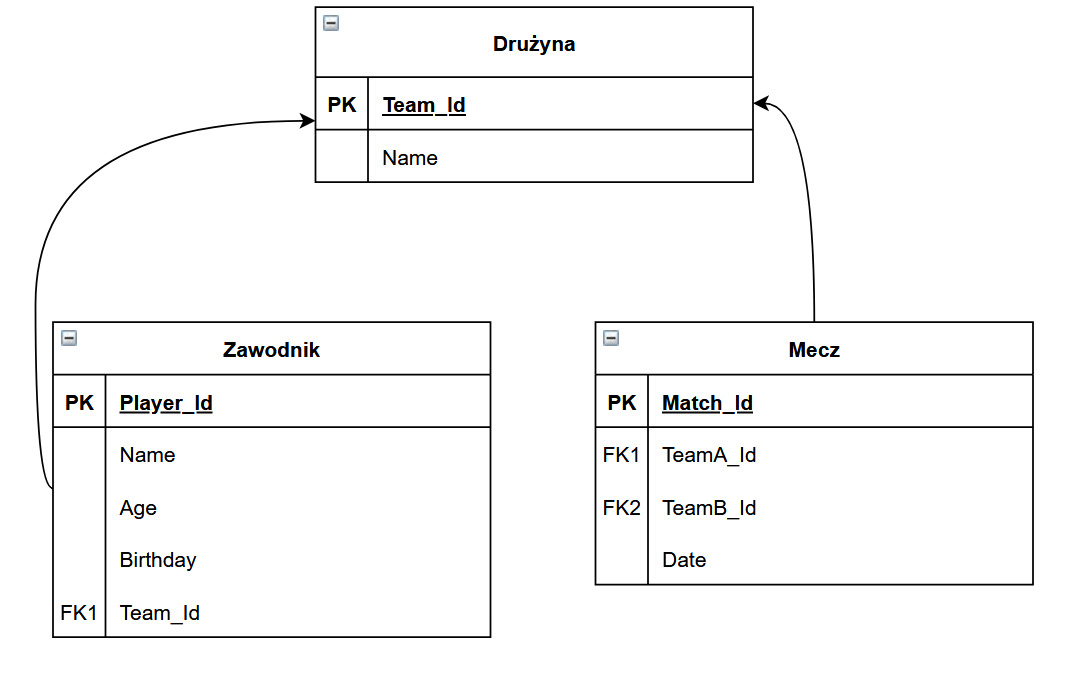
\includegraphics[width=14cm,height=10cm]{figures/Example_entities.PNG}
        \caption{Przykładowy schemat relacji encji relacyjnej bazy danych.}\label{example-Entity}
\end{figure}

Powodem dla którego nazywamy to relacyjną bazą danych jest możliwość wstawienia odnośnika jako kolumne, który wskazuje na rząd w innej tabeli. Patrząc na przykładowy schemat \ref{example-Entity}, można zauważyć, że kolumny \textit{TeamA\_Id} oraz \textit{TeamB\_Id} z tabeli \textit{Mecz}, odnoszą się do wartości w tabeli \textit{Drużyna}. Wartości w kolumnach, odwołujące się do innych tabel nazywamy \textit{kluczami obcymi}. \cite{Relational_Databases_Milan}

Obecnie istnieje duża ilość oprogramowania, umożliwiającego zarządzanie takimi bazami danych, np. \textit{Microsoft SQL Server} czy \textit{PostgreSql}, lecz wszystkie sprowadzają się do ujednoliconego standardu ISO \cite{SQL_ISO}. Zdefiniowane są tam zasady, jaką RBD powinny mieć strukturę oraz jakie typy danych zawierają. W pracy zostały użyte ze względu na łatwość dostępu do narzędzi oraz możliwości utworzenia instancji na chmurze, korzystając z Azure Cloud.

~

Problem pobierania danych dla algorytmów uczenia maszynowego został rozwiązany poprzez użycie WebAPI (\english{Web Application Programming Interfaces}). API to zbór funkcji i reguł wewnątrz aplikacji, umożliwiający interakcje z tą aplikacją za pośrednictwem oprogramowania \cite{webAPI_Mozzila}. W przypadku WebAPI korzystanie z interfejsu sprowadza się do wykonywania żądań http pod odpowiedni adres internetowy. Przykładowo, API Twitter umożliwia pobranie ostatnich wpisów podanego użytkownika, za pomocą żądania http pod udostępniony URL (\english{Uniform Resource Locator}) oraz wiele innych interakcji z stroną \cite{Twitter_API}.

Użycie WebAPI jako sposobu udostępniania danych umożliwia nam wstępnie zagregowanie danych do ujednoliconego formatu JSON (\english{JavaScript Object Notation}), dla którego istnieje wiele parserów, dzięki czemu można z nim łatwo pracować \cite{JsonParserPython}.

\section{Wstępne przetwarzanie i wizualizacja danych}

\noindent 

Jednym z kluczowych aspektów mocno wpływających na powodzenie każdego projektu związanego z uczeniem maszynowym jest stworzenie odpowiedniego zbioru cech (\english{features}) na podstawie poprawnie przygotowanych danych. W kontekście uczenia maszynowego, cecha to indywidualna, mierzalna własność lub charakterystyka pewnego obserwowanego zjawiska~\cite{Wiki:Feature}. W przypadku modelu przewidującego wyniki meczów piłkarskich, przykładem cechy może być liczba żółtych kartek uzyskanych przez drużynę gospodarzy w ostatnim meczu lub średni procent posiadania piłki drużyny gości w meczach obecnego sezonu.

Metody zbioru danych są bardzo często automatyzowane i pozbawione ścisłej kontroli, stąd mogą one zawierać różnego rodzaju błędy, takie jak wartości spoza zakresu (np. wiek: -20), niemożliwe kombinacje wartości (płeć: mężczyzna, w ciąży: tak) lub pominięte atrybuty dla niektórych rekordów. Ważne jest, aby takie błędy wychwycić już na etapie wstępnego przetwarzania i nie dopuścić ich do danych wejściowych algorytmów. Pomocna może się tutaj okazać wizualizacja dokonana w celu bliższego zapoznania się z danymi. Dla atrybutów można wizualizować rozkład ich wartości przy pomocy histogramów lub wypisywać ich podstawowe statystyki (m.in. średnie, mediany, wartości minimalne, maksymalne) w celu weryfikacji poprawności ich zakresów i typów.

System będzie w stanie nauczyć się przewidywać wyniki tylko mając do dyspozycji jak najwięcej znaczących cech i jak najmniej tych mało znaczących. Zgodnie z popularnym angielskim zwrotem w obszarze przetwarzania informacji -  \definicja{śmieci na wejściu – śmieci na wyjściu} (\english{Garbage In, Garbage Out, GIGO}), nawet skuteczny i poprawnie działający program w przypadku otrzymania na wejściu błędnych danych, da na wyjściu niepoprawne oraz mało użyteczne wyniki, stąd tak ważne jest uprzednie przygotowanie danych.

Wstępne przetwarzanie (\english{preprocessing}) w naszym systemie składa się z jednorazowego dokonania wizualizacji posiadanych przez nas danych (która będzie szczegółowo przedstawiona w późniejszym rozdziale) w celu pogłębienia wiedzy na ich temat i wyszukania potencjalnych braków lub błędów. Następnym zadaniem, wykonywanym każdorazowo przy tworzeniu zbioru danych, którego przeznaczeniem jest użycie podczas testowania różnego rodzaju algorytmów, jest pobranie interesujących danych z bazy, przetworzenie ich, czyli poradzenie sobie z m.in. wartościami pustymi i stworzenie na ich podstawie wektora cech dla każdego rekordu (w przypadku naszego systemu jest to pojedynczy mecz). 

Wynikiem etapu wstępnego przetwarzania jest tzw. zbiór treningowy (\english{training set}), którego znaczenie zostanie przybliżone w podrozdziale traktującym o algorytmach uczenia maszynowego.

\section{Algorytmy uczenia maszynowego}
Uczeniem maszynowym nazywany dziedzinę nauki (i sztukę) programowania komputerów w sposób umożliwiający im \textbf{uczenie się z danych}. \cite{Geron} Nieodłącznym elementami związanymi z tą dziedziną są takie pojęcia jak: 
\begin{itemize}
    \item zbiór treningowy (\english{training set}) - zbiór uczący zawierający dane używane do trenowania stworzonego przez nas sytemu
    \item zbiór testowy (\english{test set}) - zbiór zawierający część danych, na których dokonywana jest predykcja odpowiednich wartości przez skonstruowany system.
\end{itemize}
Warto podkreślić, że dane zawierające się w zbiorze testowym nie występują w zbiorze treningowym, co daje nam pewność, że algorytm nie będzie miał wcześniej do czynienia z danymi, na których ma wykonać predykcję aniżeli dopiero na etapie tejże predykcji.

Istnieje wiele typów uczenia maszynowego, że warto podzielić je na ogólne kategorie na podstawie takich czynników, jak:
\begin{itemize}
    \item nadzór człowieka w procesie trenowania (uczenie nadzorowane, nienadzorowane, półnadzorowane i uczenie przez wzmacnianie)
    \item możliwość uczenia się w czasie rzeczywistym (uczenie przyrostowe i wsadowe)
    \item sposób pracy: proste porównywanie punktów danych ze znanymi punktami lub, podobnie do naukowców, wykrywanie wzorców w danych uczących i tworzenie modelu predykcyjnego (uczenie z przykładów i uczenie z modelu)
\end{itemize}

Konstruowany system do predykcji wyniku meczu piłkarskiego jest przykładem systemu wykorzystującego uczenie nadzorowane. W uczeniu nadzorowanym (\english{supervised learning}) dane uczące przekazywane algorytmowi (wektor cech nt. danego meczu) zawierają dołączone rozwiązania problemu, tzw. etykiety (\english{labels}) (wynik danego meczu). \cite{Geron}

\begin{figure}[h] 
        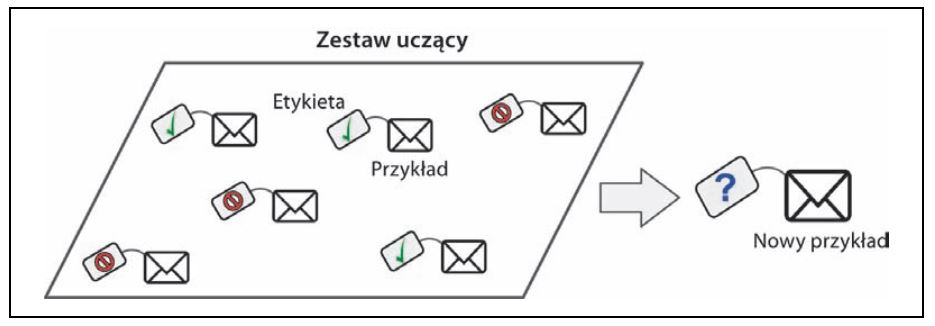
\includegraphics[width=15cm]{figures/supervised-learning.JPG}
        \caption{Zbiór danych uczących zaopatrzony w etykiety, stosowany w uczeniu nadzorowanym}
\end{figure}

\newpage

\subsection{Regresja Logistyczna}
\definicja{Regresja logistyczna} (\english{Logistic Regression}) - jedna z powszechnie używanych metod klasyfikacji. Klasyfikacja ta może być użyta, gdy próbka przypisywana jest do jednej z dwóch klas (klasyfikacja binarna) \cite{PPlonski}. Istnieją także rozszerzone modele regresji logistycznej obsługujące możliwą predykcję do więcej niż dwóch klas (klasyfikacja wieloklasowa). Regresja logistyczna oparta jest o specyficzny system prawdopodobieństw i funkcji sigmoidalnej, na podstawie której wyznaczana jest przynależność danej obserwacji do odpowiedniej klasy.

Funkcja sigmoidalna opisana jest następującym wzorem:
\begin{equation}
    f(z) = \frac{1}{1 + \exp^{-(az + b)}}
\end{equation}

gdzie:
\begin{itemize}
    \item z - wektor zmiennych niezależnych dla danej obserwacji
    \item a - wektor zawierający wagi dla odpowiednich cech
    \item b - stała regresji zapewniająca przesunięcie hiperpłaszczyzny decyzyjnej klasyfikatora w przestrzeni wag
\end{itemize}

\begin{figure}[h] 
        \centering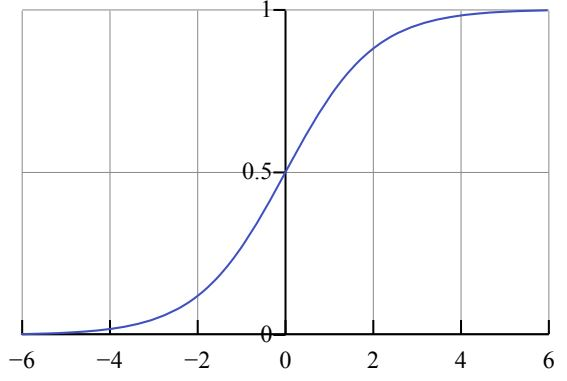
\includegraphics[width=15cm]{figures/sigmoidFunc.JPG}
        \caption{Krzywa regresji logistycznej \cite{MGrzyb}}
\end{figure}

Jak możemy zauważyć z powyższego wykresu funkcja sigmoidalna daje wynik ciągły, który następnie sprowadzany jest do wyniku binarnego:

\[
y = 
    \begin{cases}
            0,& f(z) < 0.5\\
            1,& f(z) \ge 0.5
    \end{cases}
\]

\newpage
\subsection{Las losowy}
\definicja{Las losowy} (\english{Random Forest}) - zbiór klasyfikatorów (\english{ensemble classifier}), w którym każdy pojedynczy klasyfikator jest drzewem decyzyjnym uczonym bez zatrzymywania \cite{PPlonski}. Aby zrozumieć ideę lasu losowego musimy najpierw zrozumieć ideę drzewa decyzyjnego. Drzewa decyzyjne (\english{decision trees}) opierają się o drzewiastą strukturę. Proces klasyfikacyjny budowany jest w sposób iteracyjny począwszy od korzenia aż do liści. W kolejnych iteracjach dodawane są węzły składające się z odpowiednio dobranych atrybutów. Atrybuty są wybierane przez tzw. algorytm wyboru cech, w kolejności mającej zmaksymalizować zysk informacyjny z danego węzła. Cały proces ma swój koniec w momencie, gdy wszystkie liście są w tej samej klasie lub gdy zabraknie klas do podziału. Budując pełne drzewo decyzyjne istnieje duże prawdopodobieństwo nadmiernego dopasowania algorytmu, co jest częstym problemem w przypadku podstawowej wersji drzewa decyzyjnego. \cite{MGrzyb}\\

Przykładowy model drzewa decyzyjnego:
\begin{figure}[h] 
        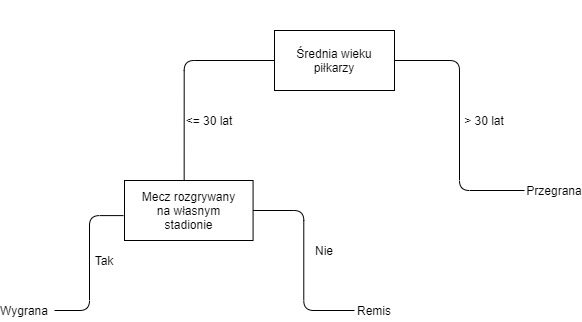
\includegraphics[width=14cm]{figures/decTree.jpg}
        \caption{Przykładowy model drzewa decyzyjnego}
\end{figure}

Na podstawie powyższego modelu jesteśmy w stanie przeprowadzić proste wnioskowanie decyzjne. Załóżmy, że nasza obserwacja wyróżnia się następującymi atrybutami:
\begin{itemize}
    \item Średnia wieku piłkarzy - 25.4 lat
    \item Mecz rozgrywany na własnym stadionie - Nie
\end{itemize}
Znamy wartości wszystkich potrzebnych do wnioskowania atrybutów wobec czego jesteśmy w stanie rozpocząć proces predykcji rozpoczynając wnioskowanie od korzenia. Średnia wieku piłkarzy jest mniejsza jak 30 lat, wobec czego trafiamy do lewej gałęzi drzewa. Kolejno sprawdzamy czy badany przez nas mecz jest rozgrywany na własnym stadionie - według badanej obserwacji mecz jest rozgrywany na wyjeździe w związku z czym odpowiadamy, że nie i kierujemy się prawą gałęzią drzewa. W tym momencie dochodzimy do liścia z etykietą ,,Remis'', która to etykieta jest naszą ostateczną predykcją wyniku meczu na podstawie wnioskowania w tym drzewie decyzyjnym.\\

Rozumiejąc ideę drzewa decyzyjnego jesteśmy w stanie przejść do omówienia algorytmu lasu losowego, który tak jak wspomnieliśmy jest zbiorem klasyfikatorów, gdzie każdy klasyfikator jest drzewem decyzyjnym. Każde drzewo wchodzące w skład lasu losowego jest uczone na specjalnie wylosowanej dla niego próbce danych pochodzącej ze zbioru uczącego, treningowego. Dodatkowo, w trakcie budowania drzewa decyzyjnego nie wszystkie atrybuty są brane pod uwagę przy wyznaczaniu reguły decyzyjnej w węźle. Losowany jest pewien podzbiór atrybutów, na podstawie których wyznaczana jest reguła decyzyjna w węźle. Obie opisane techniki działania na próbce danych i pewnym wylosowanym podzbiorze atrybutów stosowane są w celu zwiększenia stabilności odpowiedzi algorytmu i jego ochrony przed nadmiernym dopasowaniem do danych uczących, co było jedną z największych wad pojedynczego drzewa decyzyjnego i co przekłada się dodatkowo na lepszą skuteczność działania klasyfikatora na nowych danych. W trakcie przewidywania klasy dla próbki jest ona pokazywana wszystkim drzewom decyzyjnym, a jako końcowa decyzja o przynależności do klasy traktowanej jest przypisanie do klasy najczęściej wskazywanej przez drzewa decyzyjne w lesie. Dodatkowym plusem lasu losowego jest umiejętność wyznaczenia ważności atrybutów wejściowych. \cite{PPlonski}\\

Przykładowy proces wnioskowania na podstawie algorytmu lasu losowego możemy zobaczyć na poniższym obrazie
\begin{figure}[h] 
        \centering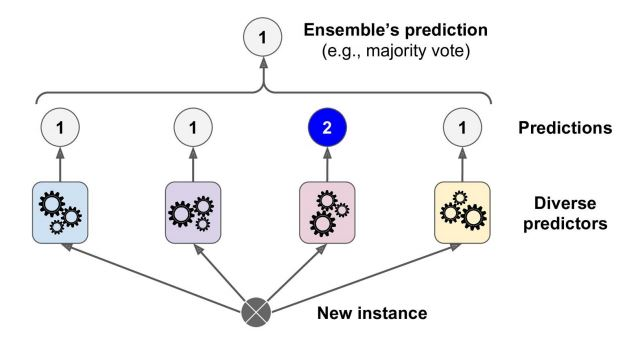
\includegraphics[width=14cm]{figures/randomForestModel.JPG}
        \caption{Przykładowy model lasu losowego \cite{Geron}}
\end{figure}

\newpage

\subsection{Metoda Wektorów Wspierających - SVM}
\definicja{Metoda wektorów wspierających - nośnych} (\english{Support Vector Machine, SVM}), jest to nadzorowana technika uczenia maszynowego wykorzystywana do zadań klasyfikacji oraz regresji. Technika ta została opracowana w laboratorium AT\&T Bell poprzez Vladimira Naumovicha Vapnika wraz ze współpracownikami (Boser i in., 1992, Guyon i in., 1993, Vapnik i in., 1997). \cite{Wiki:SVM}. Głównym założeniem tej metody jest wyznaczenie hiperpłaszczyzny, która ma za zadanie rozdzielić przy pomocy maksymalnego marginesu przykłady należące do różnych klas. W przypadku występowania więcej niż dwóch klas, metoda ta wykorzystuję technikę \definicja{OvR} (\english{One-vs-Rest}), która polega na szkoleniu jednego klasyfikatora na klasę, z próbkami z tej klasy jako pozytywne próbki, a inne próbki jako negatywy. Formalnie problem klasyfikacji przedstawia się następująco \cite{Prezentacja:SVM2}: 
\begin{itemize}
    \item W przestrzeni danych (ang. measurement space) $\omega$ znajdują się wektory danych x stanowiące próbkę uczącą D, należące do dwóch klas\\
    \begin{equation}
D = \big\{(x_{i}, c_{i}) | x_{i} \in R^{p}, c_{i} \in \{-1, 1\}\big\}_{i=1}^{N}
    \end{equation}
    \item Szukamy klasyfikatora pozwalającego na podział całej przestrzeni $\omega$ na dwa rozłączne obszary odpowiadającej klasom {1,-1} oraz pozwalającego jak najlepiej klasyfikować nowe obiekty x do klas
    \item Podejście opiera się na znalezieniu tzw. granicy decyzyjnej między klasami → g( x )
\end{itemize}
Dodatkowo dwie klasy są liniowo separowalne, jeśli istnieje hiperpłaszczyzna H postaci: \[g(x) = w^Tx + b\] przyjmująca wartości: 

\[
    \begin{cases}
            g(x_{i}) > 0,& x_{i} \in 1 \\
            g(x_{i}) < 0,& x_{i} \in -1
    \end{cases}
\]
\\

Linia granicy decyzyjnej nie tylko oddziela dwie klasy, ale także pozostaje jak najdalej od najbliższych instancji. Jak pokazano na rysunku \ref{SVM-margines} problemem poza znalezieniem $B_{2}$ jest również znalezienie szerokości wspomnianej granicy. Niestety nie ma na to idealnego rozwiązania i konieczne jest wybranie cech, które są bardziej odpowiednie dla naszego problemu. Szerszy margines to lepsze własności generalizacji, mniejsza podatność na
ewentualne przeuczenie (\english{overfitting}), a z kolei wykorzystanie wąskiego marginesu skutkuje radykalną zmianą klasyfikacji przy małej zmianie granicy. Jednak ze względu na oszacowanie górnej granicy błędu ze względu na błąd uczący częściej wybiera się jak najszerszy margines w celu lepszego uogólniania w bardziej skomplikowanych modelach.

\begin{figure}[H] 
        \centering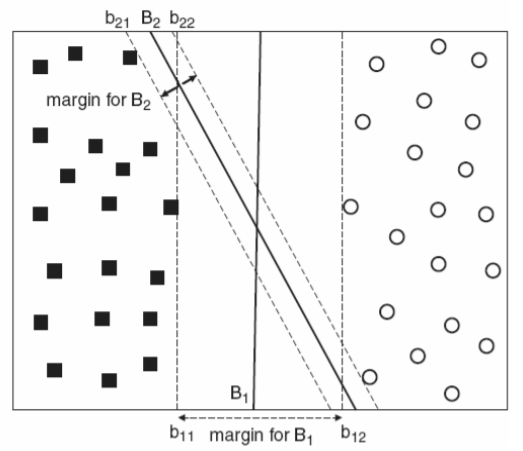
\includegraphics[width=6cm,height=6cm]{figures/SVM-margin.png}
        \caption{Margines granicy decyzyjnej}\label{SVM-margines}
\end{figure}
Konsekwentnie, problem maszyn wektorów nośnych sprowadza się do poszukiwania maksymalnego marginesu klasyfikacji: $w x + b = 0$ gdzie \definicja{w} oraz \definicja{b} są parametrami modelu.
\[
y = 
    \begin{cases}
            1,&  wx+b > 0\\
            -1,& wx+b < 0
    \end{cases}
\]
Dodatkowo parametry granicy wyznacza się tak, aby maksymalne marginesy (margines to odległość między \definicja{bi1} oraz \definicja{bi2}) \definicja{bi1} i \definicja{bi2} były miejscem geometrycznym punktów \definicja{x} spełniających warunki \ref{SVM-marginesEq}:
\[
    \begin{cases}
            bi1,&  wx+b = 1\\
            bi2,& wx+b= -1
    \end{cases}
\]
\begin{figure}[H] 
        \centering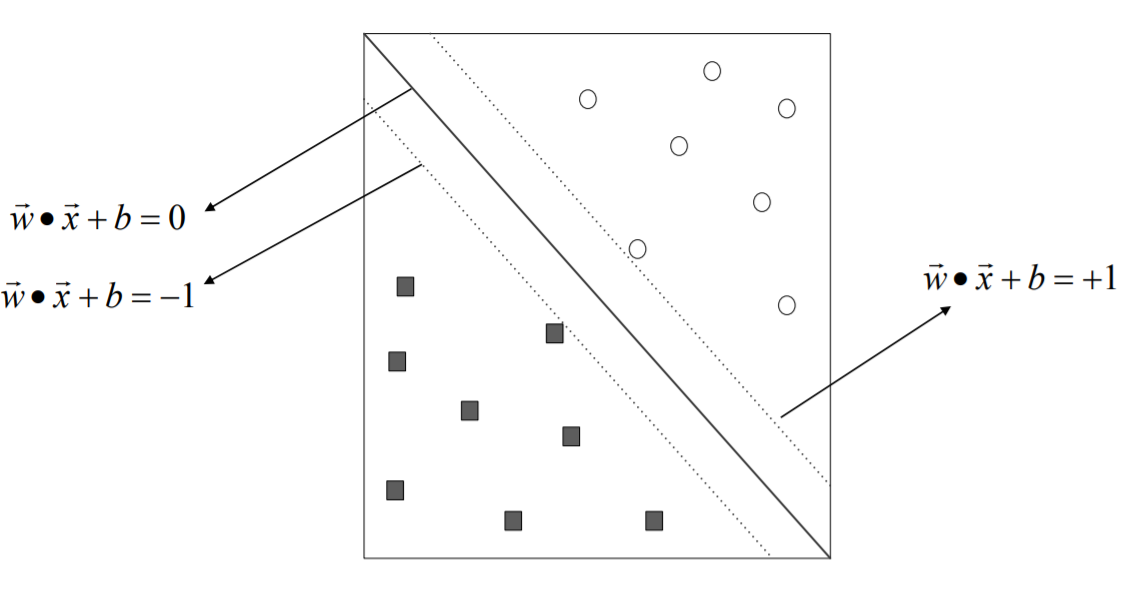
\includegraphics[width=14cm,height=6cm]{figures/SVM-marginEq.png}
        \caption{Wyznaczanie marginesu granicy decyzyjnej}\label{SVM-marginesEq}
\end{figure}

Tak więc problem ten sprowadza się do optymalizacji kwadratowej z liniowymi ograniczeniami (uogólnione zadanie optymalizacji). 
Czasami jednak mamy do czynienia z sytuacją podczas której nie mamy możliwości w pełni liniowej separacji klas. W takiej sytuacji wykorzystuje się zmienne osłabiające \definicja{$\xi_{i} \ge 0$}, które dobiera się dla każdego przykładu uczącego. Jej wartość zmniejsza margines separacji. Jeżeli $0 \le \xi_{i} \le 1$, to punkt danych $(xi,di)$ leży wewnątrz strefy separacji, ale po właściwej stronie, a w sytuacji gdy $\xi_{i} \ge 1$, to punkt leży po niewłaściwej stronie hiperpłaszczyzny i nastąpi błąd klasyfikacji. 
\[
    \begin{cases}
            bi1,&  wx+b = 1 - \xi\\
            bi2,& wx+b= -1 + \xi
    \end{cases}
\]
Również tutaj występuje konflikt doboru marginesu. Szeroki margines to dużo błędów i odwrotnie. Kończąc rozważania dotyczące liniowej maszyny wektorów nośnych, nasz problem znalezienia granicy decyzyjnej sprowadza się do minimalizacji wyrażenia:
\[
L(w) = \frac{\|\vec{w}\|}{2} + C\big(\sum_{i=1}^{N}\xi_{i}^{k}\big)
\]
z ograniczeniami:
\[
f(\vec{x_{i}}) = 
    \begin{cases}
            1 &  \text{if}\ \vec{w} \bullet \vec{x_{i}}+b \ge 1 - \xi_{i}\\
            -1 &  \text{if}\ \vec{w} \bullet \vec{x_{i}}+b \le 1 + \xi_{i}
    \end{cases}
\]
gdzie parametr \definicja{C} to ocena straty związanej z każdym błędnie klasyfikowanym punktem dla którego $\xi > 0$. Problem ten to problem dualny i istnieją techniki pozwalające na jego rozwiązanie.

Dodatkowym problemem w tej metodzie jest fakt, że najczęściej klasy nie są liniowo separowane. Jednym ze sposobów na poradzenie sobie z tym problemem jest transformowanie, projekcja danych wejściowych do przestrzeni o większej liczbie wymiarów, w której dane, z dużym prawdopodobieństwem będą separowane liniowo. Funkcja decyzyjna po przekształceniu ma się następująco:
\[
g(x) = w\varphi(x) + b
\]
Problem ten jest trudny obliczeniowo do wykonania, lecz można sobie z nim poradzić za pomocą kerneli, funkcji jądrowych. Funkcje te wywodzą się z badań liniowych przestrzeni wektorowych, przestrzeni Hilberta, Banacha. Dzięki nim można wyznaczyć potrzebne parametry do rozwiązania naszego problemu. Najczęściej stosowane jądra w metodzie maszyn wektorów nośnych to: Gaussowskie, wielomianowe i sigmoidalne. Dzięki nim, nie musimy znać funkcji transformacji, a jedynie funkcję kernela co pozwala nam na pracę w nowej przestrzeni. 

Można zauważyć, że metoda SVM jest silną metodą pozwalającą na rozwiązywanie problemów klasyfikacji w wielowymiarowej przestrzeni danych. Dzięki niej można skutecznie uogólniać nowe przykłady i przydzielać im odpowiednie klasy zdefiniowane dla konkretnego problemu.

\newpage

\subsection{Sztuczne Sieci Neuronowe - SNN}
\label{SNN-opis}

\definicja{Sztuczna sieć neuronowa} ogólna nazwa struktur matematycznych i ich programowych lub sprzętowych modeli, realizujących obliczenia lub przetwarzanie sygnałów poprzez rzędy elementów przetwarzających, zwanych sztucznymi neuronami, wykonujących pewną podstawową operację na swoim wejściu. Oryginalną inspiracją takiej struktury była budowa naturalnych neuronów, łączących je synaps, oraz układów nerwowych, w szczególności mózgu \cite{Wiki:SNN}. Sztuczne sieci neuronowe charakteryzują się tym, że mają zdolność do odwzorowania różnych zależności pomiędzy sygnałami wejściowymi i wyjściowymi. Sztuczna sieć neuronowa składa się z wielu połączonych neuronów, a kady neuron można interpretować jako pewna kombinacja matematyczna cech wejściowych wraz z przypisanymi im wagami. Wyjście neuronu to pewna funkcja matematyczna, która przekształca daną kombinację danych wejściowych i przekazuje taki wynik na swoje wyjście. Graficzna reprezentacja takiego neuronu ma się następująco \cite{Prezentacja:SNN} \cite{KrawiecStefanowski03} --- \textbf{to jest także ze skryptu KKJS}:
\begin{figure}[H] 
        \centering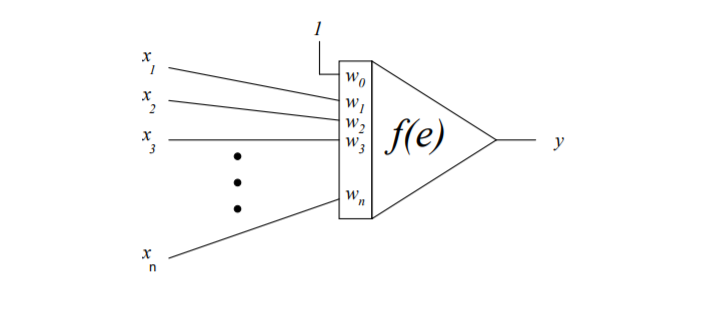
\includegraphics[width=12cm,height=6cm]{figures/SNN.png}
        \caption{Sztuczny neuron}\label{SVM-neuron}
\end{figure}

Podstawowe elementy składowe: 
\begin{itemize}
    \item n wejść neuronu wraz z wagami $w_{i}$ (wektor wag w i wektor sygnałów wejściowych x)
    \item jeden sygnał wyjściowy y
    \item pobudzenie e neuronu jako suma ważona sygnałów wejściowych
pomniejszona o próg $\Theta$
\[
e = \sum_{i=1}^{N} w_{i} x_{i} - \Theta = w^{T} x - \Theta
\]
wprowadźmy wagę $w_{0}= \Theta$, podłączonej do stałego sygnału $x_{0} = 1$;
wówczas: 
\[
e = \sum_{i=0}^{N} w_{i} x_{i}  = w^{T} x
\]
\item funkcja aktywacji (przejścia):
\[
y = f(e)
\]
\end{itemize}
Kluczowe znaczenie dla działania neuronu ma funkcja aktywacji. Mamy do wyboru liniową funkcję lub nielinową (ciągła i nieciągła, unipolarna i bipolarna).

W literaturze wyróżnia się dwa ogólne typy sieci neuronowych i są to: jednokierunkowe SNN oraz rekurencjne SNN (sieci ze sprzężeniami zwrotnymi np. sieć Hopfielda albo sieci uczenia się przez współzawodnictwo).
Sieci jednokierunkowe to sieci o jednym kierunku przepływu sygnałów. Szczególnym przypadkiem architektury jednokierunkowej jest sieć warstwowa, reprezentująca zdecydowanie najpopularniejszą topologię.
\begin{figure}[H] 
        \centering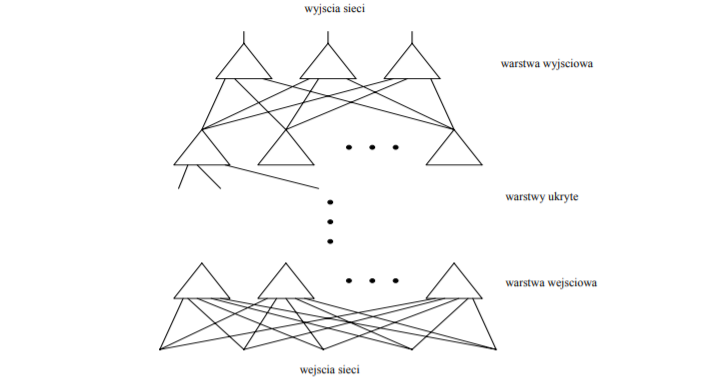
\includegraphics[width=12cm,height=6cm]{figures/ArchitekturaSNN.png}
        \caption{Sieć warstwowa jednokierunkowa}\label{SVM-neuron}
\end{figure}

Zasady łączenia neuronów między sobą:
\begin{itemize}
    \item każdy neuron z każdym,
    \item połączenia między kolejnymi warstwami w sieciach warstwowych,
    \item tylko z pewną grupą neuronów, najczęściej z tzw. sąsiedztwem
\end{itemize}

W celu uzyskania wyników wykorzystuje się \definicja{uczenie nadzorowane}. Dany jest zbiór przykładów uczących składający się z par wejście-wyjście $(x_{j}, z_{j})$, gdzie $z_{j}$ jest pożądaną odpowiedzią sieci na sygnały wejściowe $x_{j} (j=1,..m)$. Zadaniem sieci jest nauczyć się możliwie jak najdokładniej funkcji przybliżającej powiązanie wejścia z wyjściem. Odległość pomiędzy rzeczywistą a pożądaną odpowiedzią sieci jest
miarą błędu używaną do korekcji wag sieci. Typowym przykładem jest uczenie sieci wielowarstwowej algorytmem wstecznej propagacji błędu; każdy neuron lokalnie zmniejsza swój błąd stosując metodę spadku gradientu.

W celu uczenia sieci neuronowych wykorzystuje się kilka reguł i są nimi między innymi: \definicja{reguła Widrowa-Hoffa} oraz \definicja{reguła delta}. Pierwsza z nich dotyczy uczenia nadzorowanego sieci jednokierunkowych, gdzie minimalizuje się błąd pomiędzy pożądaną a aktualną odpowiedzią. 
\[
\delta^{j} = z^{j} - y^{j} = z^{j} - w^{T}x^{j}
\]

Korekta wag jest następująca \cite{Widrow}:
\begin{equation}
\label{eqn:delta}
\delta w_{i} = \eta \delta^{j} x^{j}_{i}
\end{equation}
Reguła delta z kolei obowiązuje dla neuronów z ciągłymi funkcjami aktywacji i nadzorowanego trybu uczenia. Regułę delta wyprowadza się jako wynik minimalizacji kryterium błędu średnio-kwadratowego Q.
\[
    Q = \frac{1}{2}\sum_{j=1}^{N} \big( z^{j} - y^{j}\big)^{2} = \sum_{j}^{N}Q^{j}, Q^{j} = \frac{1}{2}(\delta^{j})^{2}
\]

Korekta wag:
\[
\delta w_{i} = \eta \delta^{j} (1 - y^{j}) f'(e^{j}) x^{j}_{i}
\]
gdzie $f'()$ oznacza pochodną funkcji aktywacji. Stosowana jest do uczenia wielowarstwowych sieci neuronowych wraz z algorytmem wstecznej propagacji błędów \cite{Rumelhart}. Sieci charakterystyczne cechują się pewnymi właściwościami \cite{Mitchell}:
\begin{itemize}
    \item Przykłady uczące opisane są przez pary atrybut-wartość (na ogół
zdefiniowanych na skalach liczbowych,
    \item Przybliżana funkcja może mieć wartości dyskretne lub rzeczywiste;
może być także wektorem wartości,
 \item Dane mogą zawierać błędy lub podlegać zniekształceniu. SSN są
odporne na różnego rodzaju uszkodzenia danych, 
    \item Akceptowalny jest długi czas uczenia sieci,
    \item Akceptacja dla potencjalnie dużej liczby parametrów algorytmu,
które wymagają dostrojenia metodami eksperymentalnymi,
    \item Zadanie nie wymaga rozumienia przez człowieka funkcji
nauczonej przez SNN - trudności z interpretacją wiedzy nabytej
przez sieć (rozwijający się w tym momencie sektor uczenia maszynowego XAI - \english{explainable artificial intelligence}).
\end{itemize}

Jednak kluczowym konceptem sprawiającym, że sztuczne sieci neuronowe są tak popularne i oferujące wiele możliwości jest wsteczna propagacja błędów, czyli sposób w jaki sieć nabywa umiejętności generalizowania danych i przyporządkowywania odpowiednich wartości. Błąd k-tego neuronu w l-tej warstwie jest równy sumie błędów popełnionych przez neurony (p) z warstwy l+1-szej ważonych po wagach $w_{k(p,l+1)}$ łączących ten neuron z neuronami tej warstwy \cite{Prezentacja:SNN}: 

\[
\delta_{(k,l)}^{j} = \sum_{p=1}^{N_{l+1}} W^{j}_{k(p, l+1)} \delta_{(p,l+1)}^{j}
\]

Na podstawie wstecznej propagacji błędów, sieci neuronowe modyfikują wagi dla każdego neuronu dopowiadające danym wejściowym w celu minimalizacji funkcji nazywanej \definicja{funkcją straty}.

Wartości początkowe wag muszą być zainicjowane przed przystąpieniem do procesu uczenia i zazwyczaj dokonuje się tego w sposób losowy lub na podstawie pewnego rozkładu prawdopodobieństwa. Kluczowym czynnikiem do prędkości oraz jakości otrzymywanych wyników jest współczynnik $\eta$, który już mogliśmy zauważyć w równaniu \ref{eqn:delta}. Decyduje on o wpływie błędu popełnianego przez neuron na korektę wartości wag. Właściwy dobór ma kluczowe znaczenie dla prędkości zbieżności algorytmu, a jego zbyt mała wartość spowalnia proces uczenia i zwiększa ryzyko
wpadnięcia w pułapkę lokalnego minimum \cite{Prezentacja:SNN}. 

W momencie gdy ludzie zaczęli interesować się tematem uczenia maszynowego oraz sieciami neuronowymi zaczęto szerzej zgłębiać temat stawiając coraz to trudniejsze wyzwania. Powstało mnóstwo różnych struktur sieci. Te bardzo głębokie składające się z kilkunastu, a nawet kilkuset warstw ukrytych oraz sieci, które przyjęły trochę inną koncepcję przetwarzania danych. Jednym z dużych zmian, jakie nastąpiły w kwestii przetwarzania obrazów, było zastosowanie konwolucyjnych sieci neurnowych (\english{convolutional neural network})\cite{CNN}. Struktura takiej sieci różni się od podstawowej koncepcji tym, że zamiast w pełni połączonych warstw neuronów, posiada ona \definicja{konwolucyjne warstwy}, które mają za zadanie znalezienie pewnych wzorców na obrazie - tych większych jak i tych mniejszych. Wiele zastosowanych filtrów skanujących obraz wraz z połączeniem warstwową łączącą (\english{pooling layer}) daje w rezultacie o wiele większą skuteczność w dziedzinie przetwarzania obrazów dzięki wydobywaniu z obrazów pewnych zależności oraz połączeń pomiędzy pikselami tworzącymi obiekt \cite{Prezentacja:KKCNN} \cite{Prezentacja:CNNintro}.
Inną koncepcją w głębokich sieciach neuronowych jest struktura zwana \definicja{Rekurencyjna sieć neuronowa}  \cite{Prezentacja:KKRNN}. Główną myślą w tej koncepcji było zastosowanie zwykłej głębokiej sieci neuronowej, lecz dodatkowo, poza zwykłymi połączeniami w przód, zastosowane zostały połączenia odwołujące się również do poprzednich warstw w strukturze sieci. Dzięki takiemu rozwiązaniu można było nauczyć sieć pewnych powtarzających się wzorców, które dzięki rekurencyjnym połączeniom były łatwiejsze do wykrycia \cite{Geron2}. Dodatkowo, aby zwiększyć ilość informacji, która zostanie zapamiętana przez daną strukturę sieci, zostały wprowadzone pewne jednostki, nazywane komórkami pamięci (\english{memory cell}), takimi jak \definicja{LSTM} \cite{LSTM} czy \definicja{GRU} \cite{GRU}. Technika ta otwarła wiele możliwości w przetwarzaniu szeregów czasowych oraz pozwoliła na rozpoczęcie pracy nad przetwarzaniem języka naturalnego.

Poza wymienionymi powyżej przykładami, które różniły się budową od w pełni połączonej sieci neuronowej, powstało wiele różnych koncepcji, które były tworzone z myślą o konkretnych zastosowaniach i nie sposób opisać w tym akapicie wszystkich pomysłów.

Niestety sieć neuronowa jest trudnym narzędziem i występuję w niej problem doboru wielkości warstw ukrytych, który do teraz jest problemem otwartym. 
Nie istnieje jednoznaczna reguła określająca optymalny rozmiar danej warstwy oraz ilości warstw w danej sieci przy danym zbiorze uczącym. Zbyt mała wielkość warstw czyni sieć niezdolną do adaptacji do
zadanego zbioru przykładów co skutkuje, że w trakcie uczenia błąd
średnio-kwadratowy utrzymuje dużą wartość. Zbyt duże warstwy z kolei mają problem z przeuczaniem (nauka konkretnych wartości danych wejściowych, a nie ogólnego konceptu, zarysu) \cite{Prezentacja:SNN}.

Od początku historii SNN do teraz powstało mnóstwo konceptów, pomysłów, sztuczek i schematów które zapewniają lepsze generalizowanie, szybsze zbieganie do minimum, które nie sposób zebrać i opisać w jednym miejscu. Wiele technik zapewniło uczenie bardzo dużych sieci neuronowych zapewniających stabilne gradienty (jednym z problemów podczas nauki SNN jest niestabilność gradientów, które zanikały wraz z postępem algorytmu lub wręcz eksplodowały do bardzo dużych wartości) \cite{gradient}. Powstało również wiele funkcji aktywacji oraz sposobów inicjalizacji początkowych wag sieci.

\section{Sposób oceny wyników predykcji}
\label{section:ocenaWynikow}

Różne algorytmy dają wyniki w różnych formatach. Przy pomocy jednych uzyskujemy tylko konkretną klasę, do której przynależy konkretne wejście, a inne przyporządkowują rozkład prawdopodobieństwa możliwych wyników klasyfikacji. W naszym przypadku mamy do czynienia z obiema sytuacjami. Podczas doboru sposobu oceny algorytmów głównym celem jest dobranie takich miar, aby móc wzajemnie porównywać zastosowane algorytmy i na tej podstawie dobrać najlepsze podejście. Ocena jakości rozwiązań opierała się zatem na policzeniu \definicja{dokładności} (\english{accuracy}) na zbiorze testowym (wynoszącym 10\% całego zbioru danych), macierzy pomyłek oraz wynikające z niej miary takie jak: \definicja{precyzja} (\english{precision}, interpretować ją można jako stosunek tp / (tp + fp), gdzie tp to liczba poprawnie sklasyfikowanych przykładów, a fp to liczba niepoprawnie sklasyfikowanych przykładów.), \definicja{czułość} (\english{recall}, interpretować można jako stosunek tp / (tp + fn), gdzie tp jest liczbą poprawnie sklasyfikowanych przykładów, a fn liczbą niepoprawnie sklasyfikowanych przykładów.) oraz \definicja{F-score} (\definicja{F-score} interpretuje się jako ważoną średnią harmoniczną precyzji i czułości, gdzie wynik \definicja{F-score} osiąga najwyższą wartość przy 1, a najniższą przy 0), którą wyznaczono przy użyciu średniej typu „macro” (oblicza metryki dla każdej etykiety, a następnie wyznacza ich nieważoną średnią. Metoda ta nie uwzględnia niezbalansowania danych) \cite{SKfscore}. Dodatkowo w celu porównania zastosowana została macierz pomyłek, której schemat można zobaczyć w tabeli \ref{tab:macierz}

\begin{center}
\begin{table}[H]
\renewcommand{\arraystretch}{1.5}
\caption{Macierz pomyłek dla problemu klasyfikacji}
\label{tab:macierz}
\begin{center}
\begin{tabular}{|c|c|c|c|c|}
   \cline{3-5} 
   \multicolumn{1}{c}{} & & \multicolumn{3}{c|}{Predicted} \\ \cline{3-5}
   \multicolumn{1}{c}{} & & Draw & HomeWin & AwayWin \\ \hline
   
   {Observed}
   & Draw & T & F & F \\ \cline{2-5}
   & HomeWin & F & T & F  \\ \cline{2-5}
   & AwayWin & F & F & T \\ \hline
\end{tabular}
\end{center}
\end{table}
\end{center}

Dodatkowo przetestowano algorytmy w sposób, w którym dane wejściowe podzielono na bloki następujące po sobie. Następnie wyuczono algorytmy na pierwszym bloku i testowano jego działanie na mniejszym bloku, który w zbiorze danych występował zaraz po bloku uczącym. Kolejno do dotychczasowego zbioru uczącego dołożono dane z poprzedniego bloku testowego i na podstawie nowego zbioru znów dokonano uczenia maszynowego by następnie dokonać ewaluacji na kolejnym fragmencie zbioru testowego. Proces ten powtarzano, aż do wykorzystania wszystkich dostępnych i przygotowanych danych.


\chapter{Projekt systemu Soccer Match Predictor}

\noindent Podczas projektowania systemu trzeba było podjąć decyzje na jakie komponenty powinien zostać podzielony. Ze względu na różnorodne źródła danych, pierwszym krokiem było połączenie ich w jeden spójny zbiór. W tym celu powstała baza danych Microsoft SQL Server, która jest dostępna na platformie Azure Cloud dla każdego potencjalnego użytkownika. Baza jest przeniesiona z bazy danych SQLite \cite{kagggle_european_soccer_database}, ale musiała zostać uzupełniona innymi źródłami danych. W tym celu utworzona została konfigurowalna aplikacja konsolowa.

Kolejną decyzją do podjęcia był transfer danych z przygotowanego źródła, do skryptów przygotowujących cechy dla algorytmów uczenia maszynowego. Komponentem do tego wykorzystywanym jest aplikacja internetowa, utworzona jako WebAPI. Założone zostało, że zapytania do bazy danych powinny zostać wykonane na niezależnym poziomie, aby umożliwić wykorzystanie zasobów platformy Azure Cloud.

W celu rozdzielenia algorytmów i przygotowywania cech, które otrzymają one na wejściu, powstała biblioteka w utworzona w języku Python. Dzięki temu twórcy algorytmów uczących mogą niezależnie otrzymywać jednolicie przetworzone dane.

Wszystkie te komponenty są zapleczem dla głównego celu systemu, czyli środowiska w którym użytkownik będzie mógł skorzystać z wcześniej przygotowanych danych i algorytmów. Jest nim interaktywny \textit{Jupter Notebook}, który jest narzędziem do wykonywania predykcji przez utworzone algorytmy.

Cały system przedstawia schemat widoczny na rysunku \ref{fig:arch1}.
\newpage

\section{Ogólny schemat systemu i jego architektura}
\label{arch}
    \begin{figure}[h] 
        \centering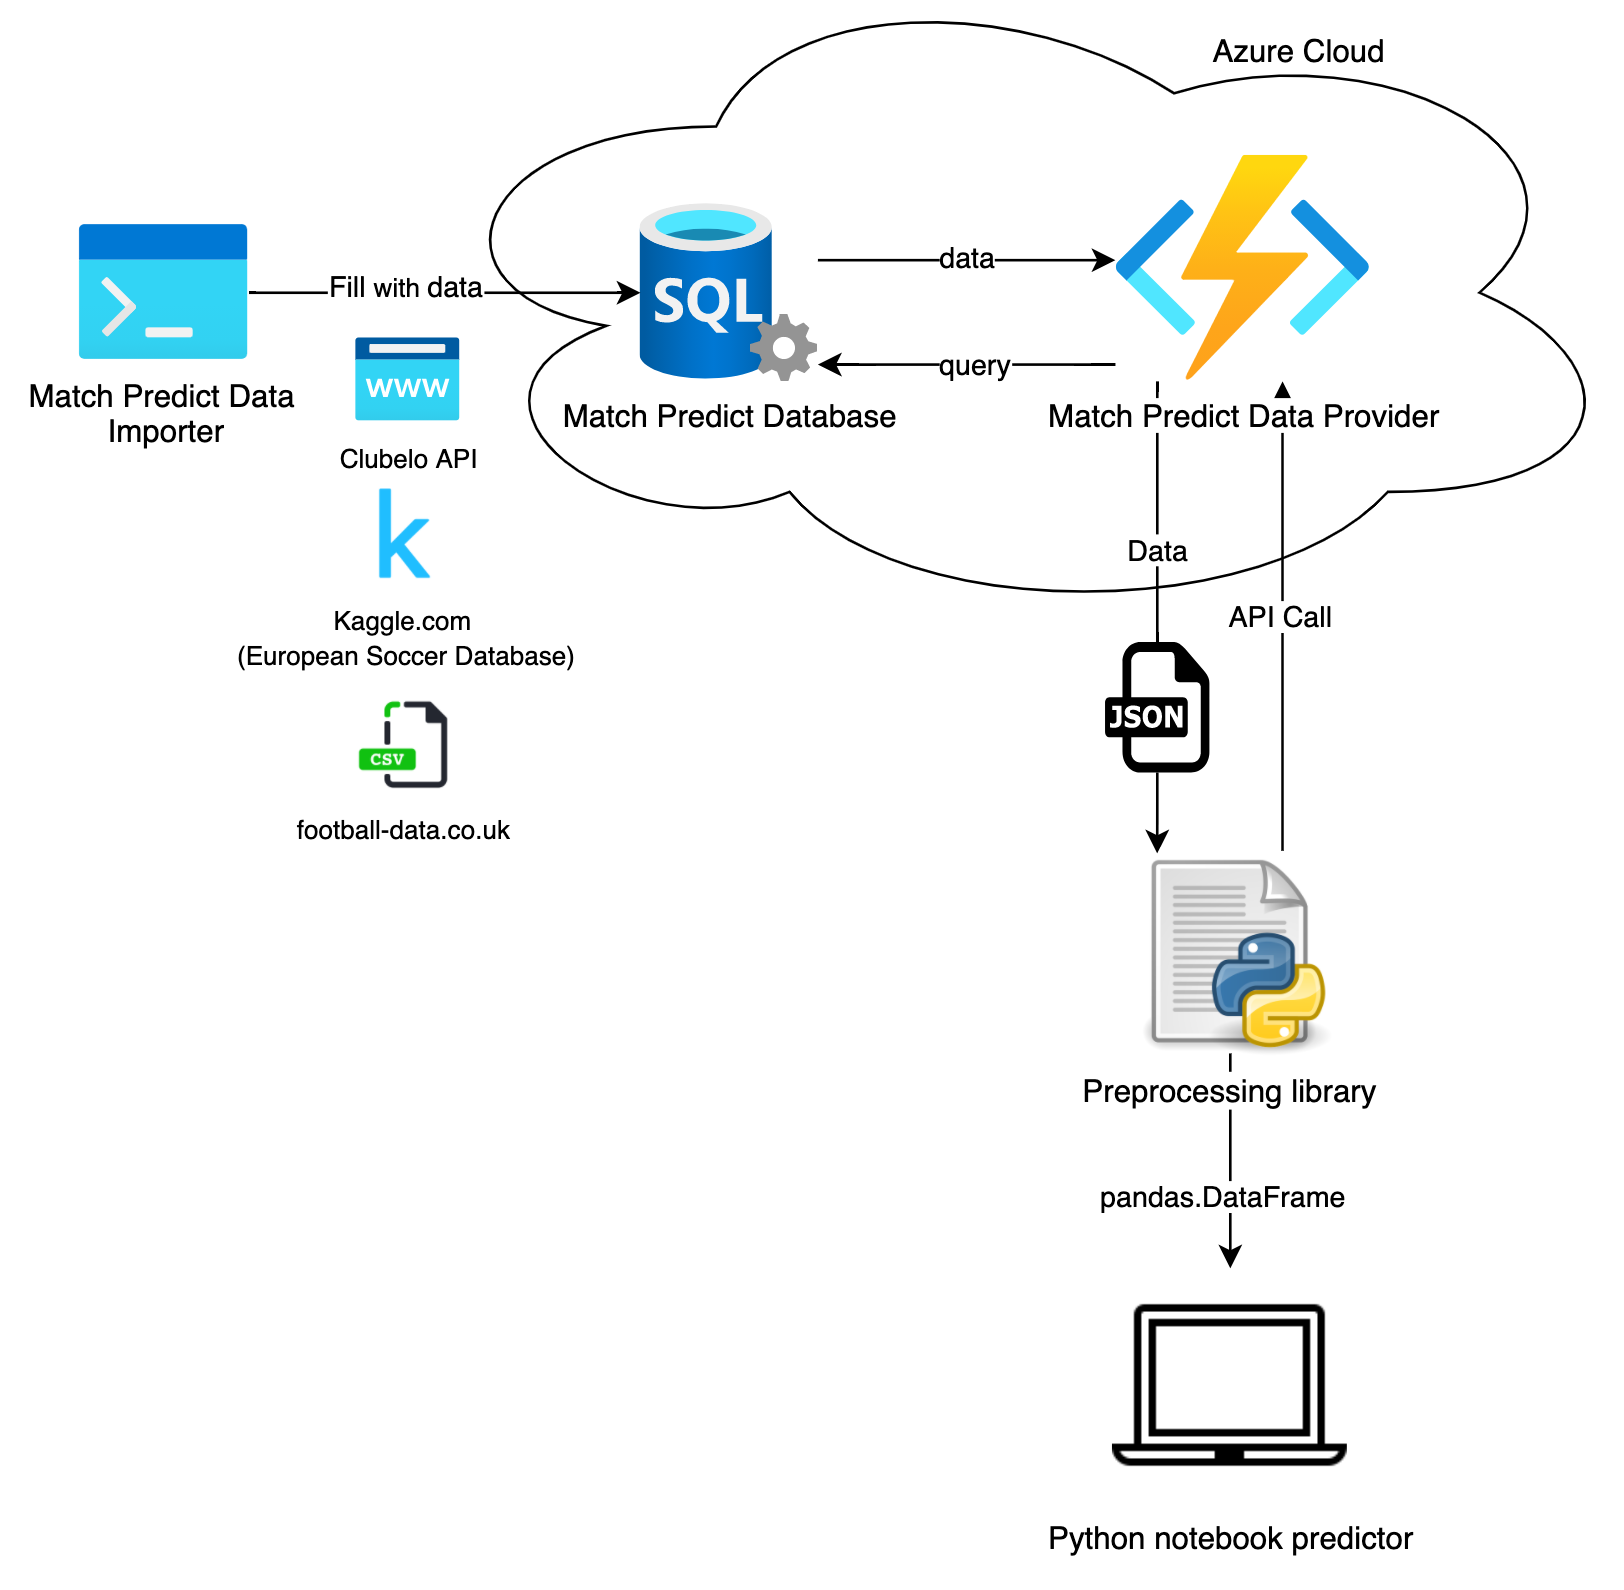
\includegraphics[width=\textwidth]{figures/MatchPredictorArchitecture.png}
        \caption{Architektura systemu Soccer Match Predictor}
        \label{fig:arch1}
    \end{figure}
\newpage

\noindent Pierwszym komponentem jest \textbf{Match Predict Data Importer}, dalej nazywany \definicja{MPDI}. Jest to aplikacja konsolowa napisana w języku C\#, której zadaniem jest import danych z różnych źródeł do docelowej bazy danych widocznej na schemacie jako \textbf{Match Predict Database}.

Baza jest przechowywanym na chmurze Azure komponentem Microsoft SQL Server, w której przechowywane są wszelkie dane wykorzystywane dalej w systemie. Schemat bazy danych jest przedstawiony w sekcji \ref{database_schema}.

Match Predict Data Provider (dalej zwany \definicja{MPDP}) służy w produkcie jako WebAPI, które przesyła dane w formacie JSON. Dane pochodzą z bazy Match Predict Database i są odpowiednio agregowane. Komponent ten to aplikacja Azure Function napisana w języku C\#, która znajduje się na chmurze Azure.

~

Kolejnym komponentem w systemie widocznym na schemacie jako \textbf{Preprocessing library} jest biblioteka służąca do pobierania danych i ich wstępnego przetwarzania wraz z tworzeniem zbioru cech. Jest to moduł napisany w języku Python, który może być wykorzystany w dowolnej aplikacji napisanej w tym języku. Komunikuje się on z opisaną wyżej bazą danych przy pomocy udostępnionego przez nią interfejsu WebAPI i otrzymuje od niego dane w formacie JSON, natomiast korzystającym z niego klientom przekazuje wygodne do operowania dane w formacie \definicja{pandas.DataFrame}. 

Uniwersalność tego modułu polega na tym, że całkowicie chowa on szczegóły implementacji swoich operacji pobierania danych z bazy, przetwarzania ich i tworzenia cech i udostępnia jedynie metody pozwalające na pobranie danych dla konkretnych sezonów i/lub konkretnych drużyn. Dzięki temu klient korzystający z tego modułu jest niezależny od wszelkich zmian strukturalnych w bazie danych czy interfejsie służącym do komunikacji z nią.

~

Ostatnim elementem jest widoczny na schemacie \textbf{Python notebook predictor}, który służy jako środowisko testowe do porównywania różnego rodzaju algorytmów stosując różne podejścia i techniki. Jest to aplikacja stworzona w \textit{Jupter Notebook}, czyli rozbudowanym narzędziu uruchamianym w przeglądarce internetowej pozwalającym na m.in. separowanie poszczególnych części kodu i uruchamianie ich niezależnie od siebie. Pozwala to na przykład na jednorazowe pobranie danych na samym początku i wielokrotne użycie ich w późniejszych eksperymentach.

Środowisko to jest klientem opisanego wyżej modułu do wstępnego przetwarzania danych i korzysta z niego do pobierania przetworzonych danych. 

\newpage
\section{Schemat bazy danych}
\label{database_schema}
\begin{figure}[h]
  \centering
   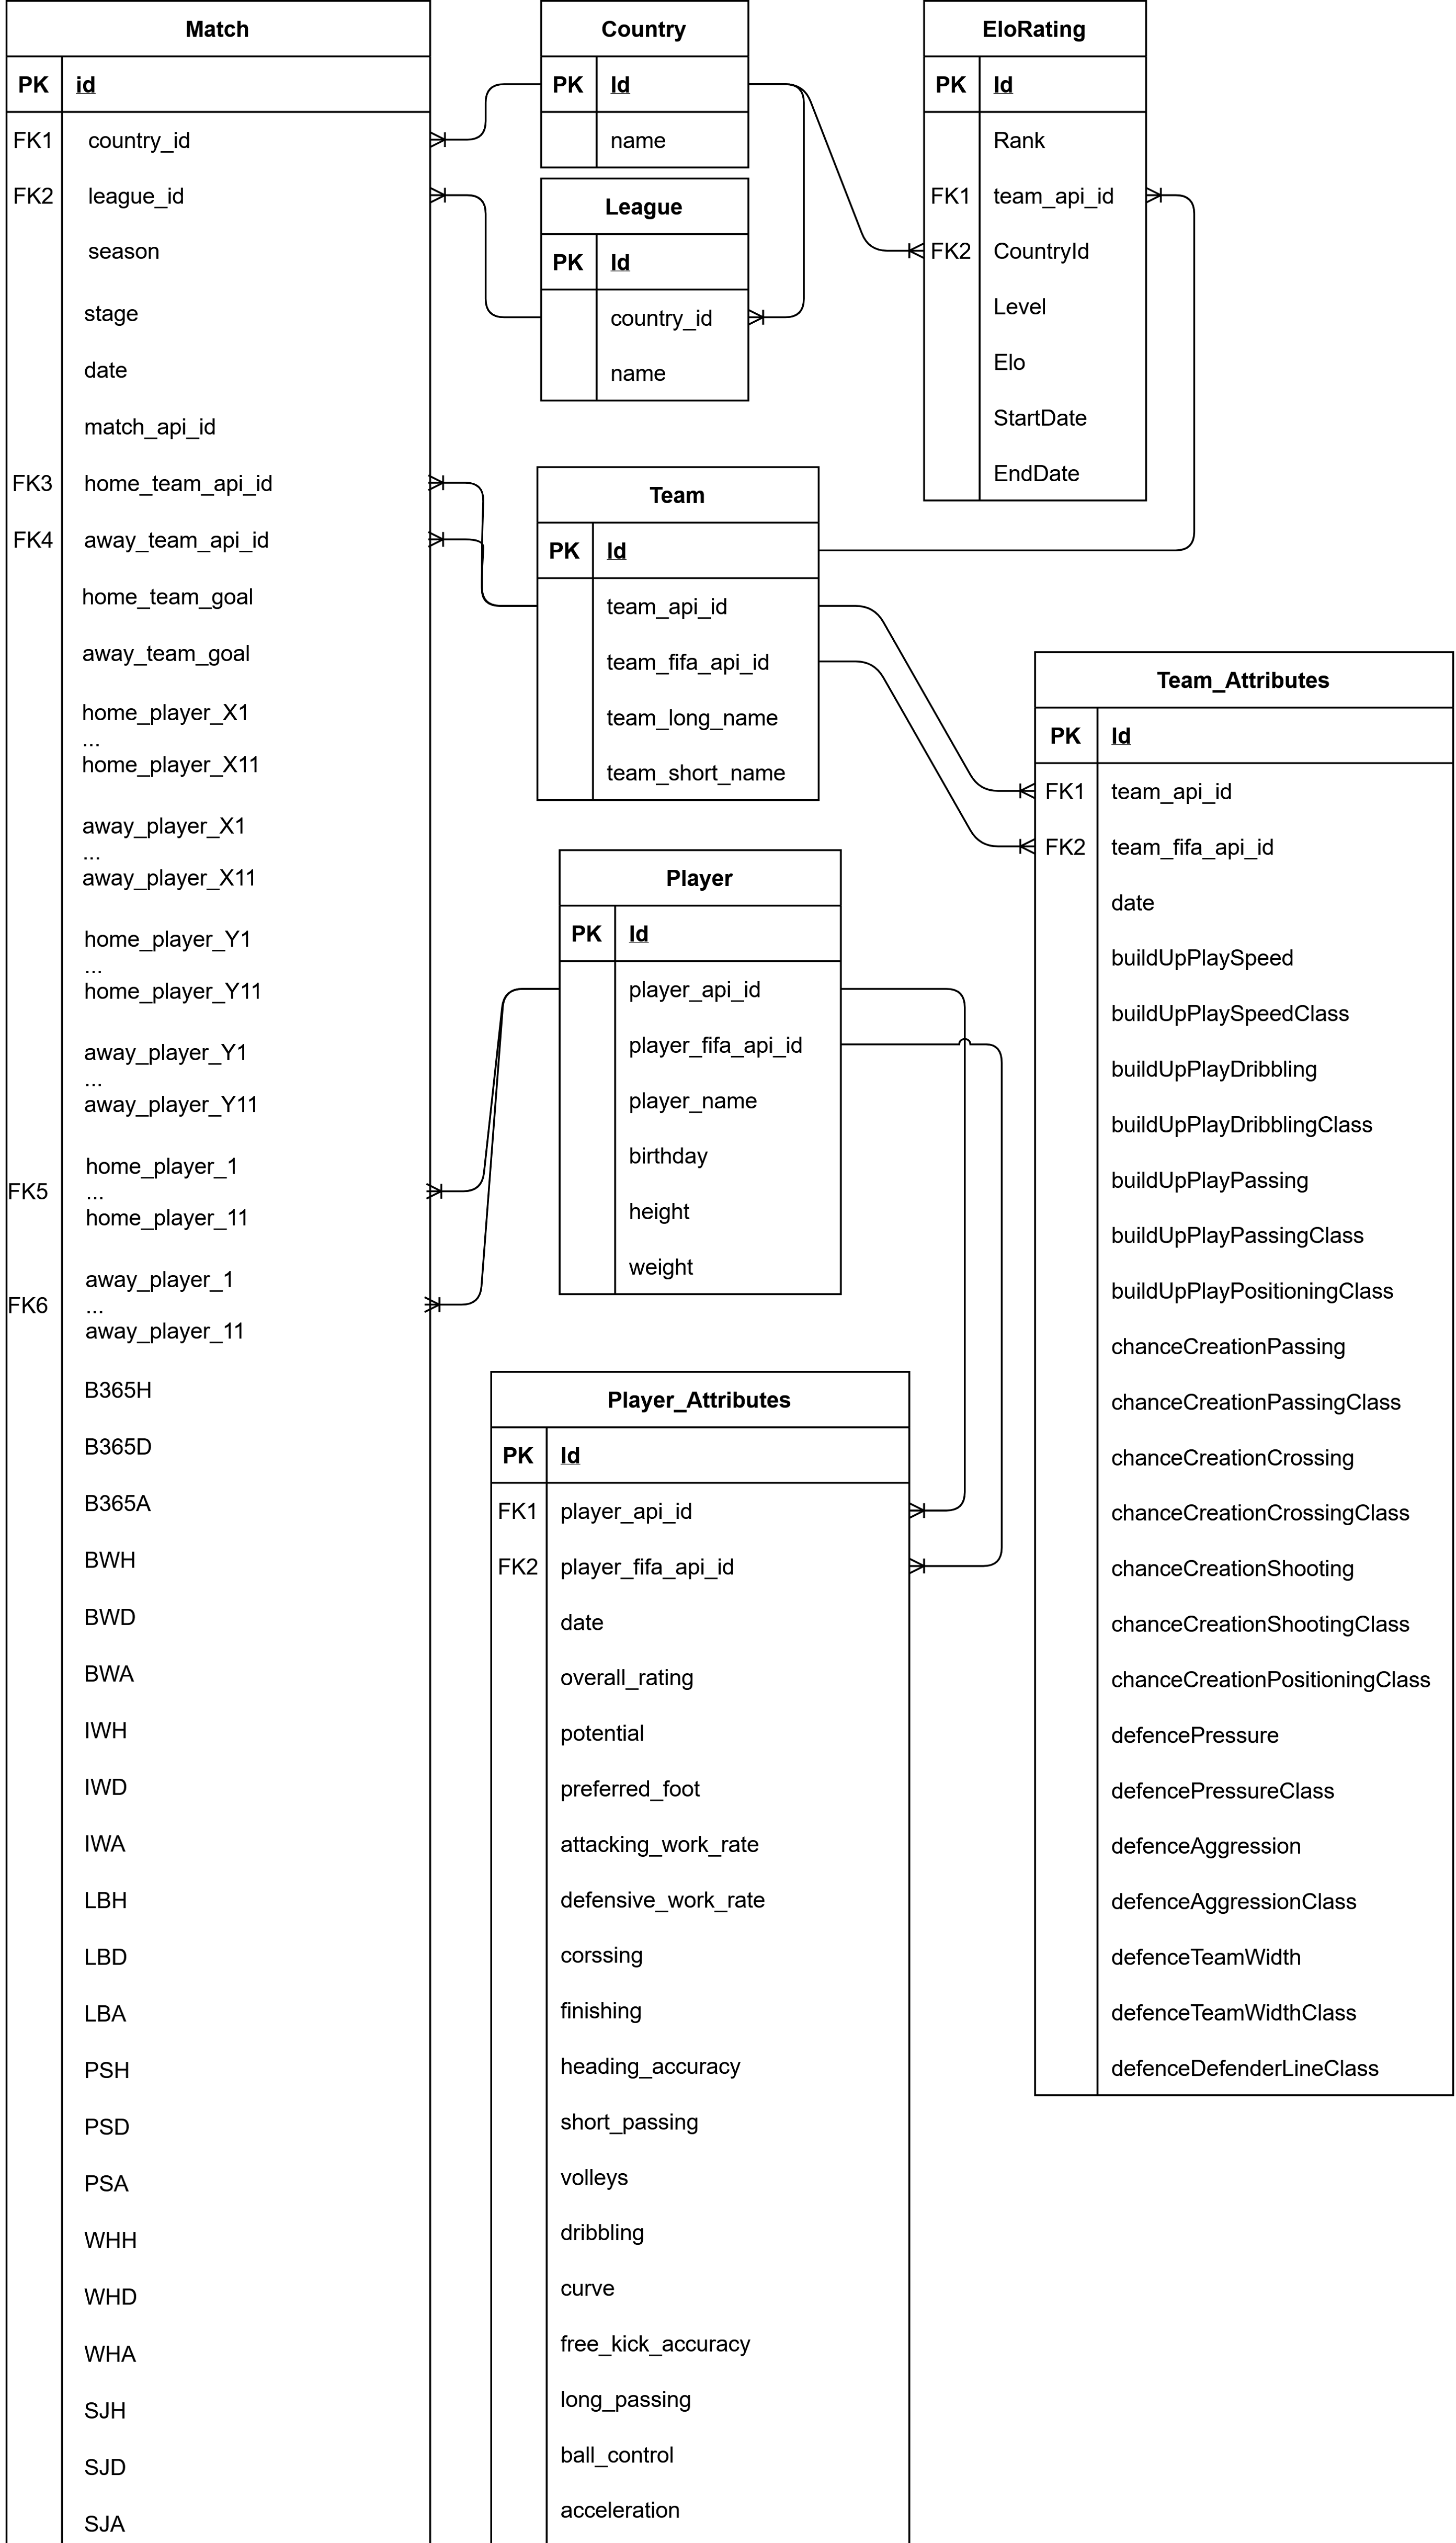
\includegraphics[width=0.83\textwidth]{figures/match_predict_schema_1.png}%

\end{figure}
\newpage
\begin{figure}[h]
\ContinuedFloat
    \centering
  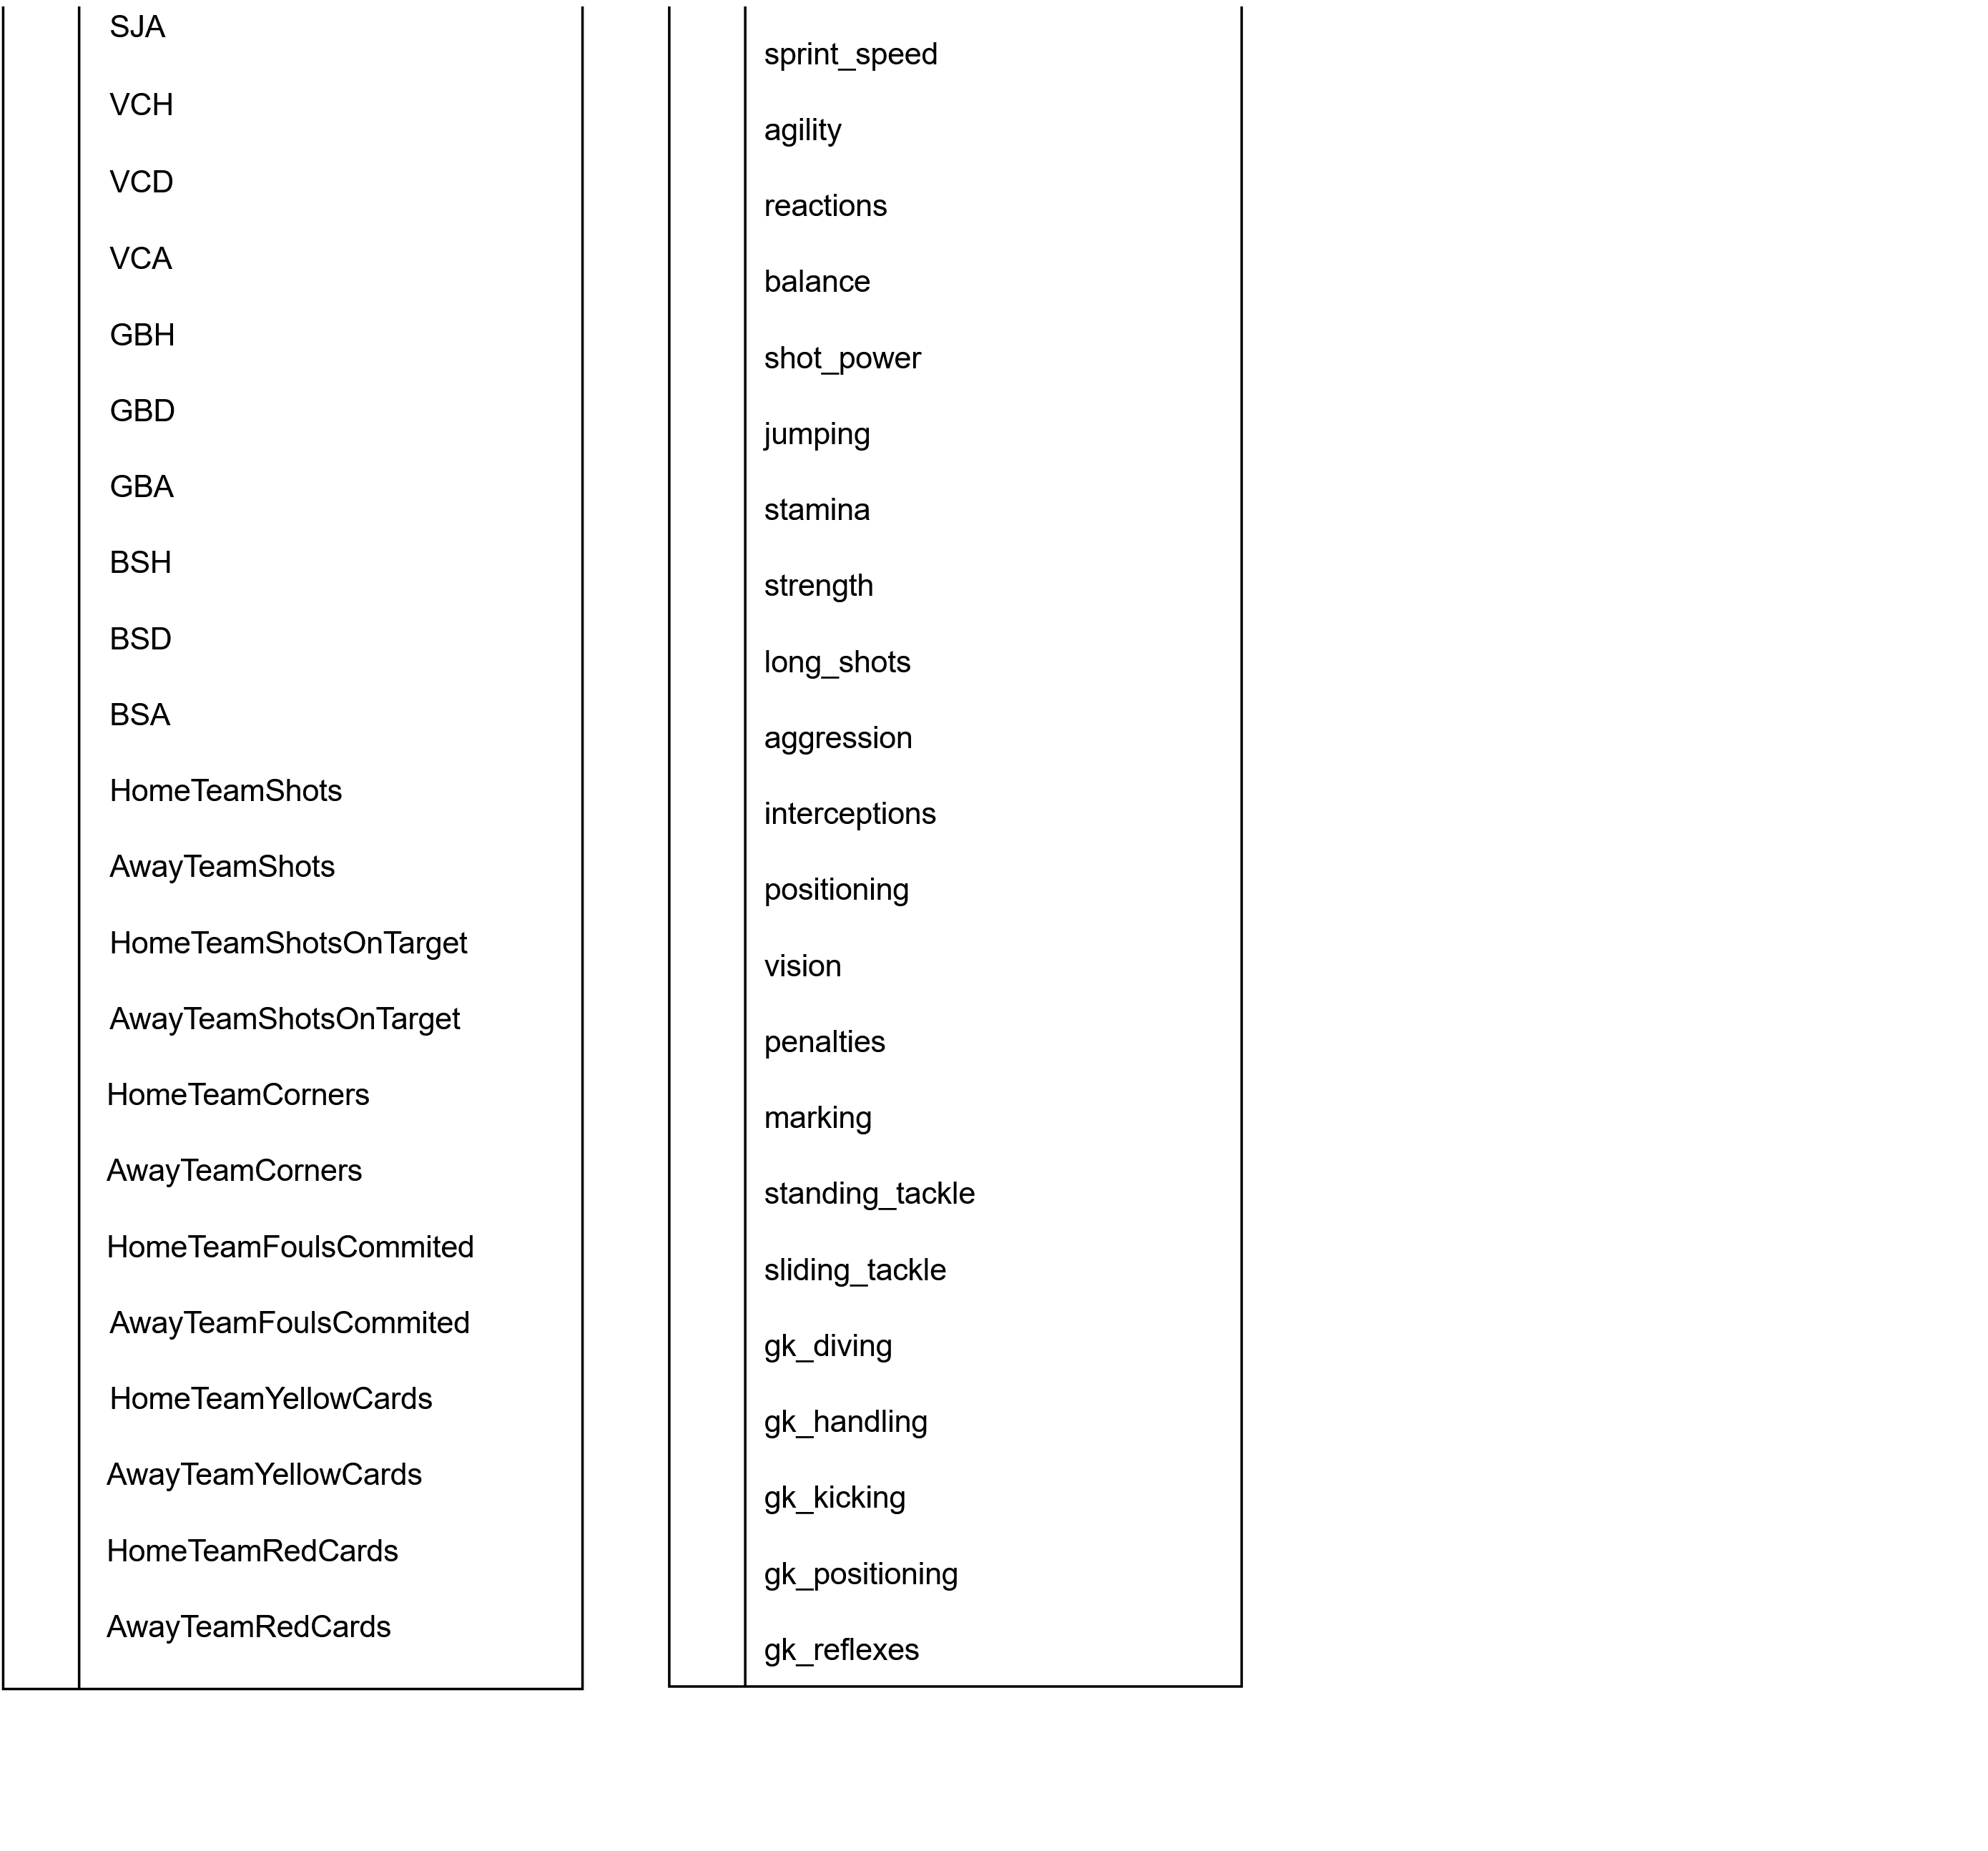
\includegraphics[width=0.83\textwidth]{figures/match_predict_schema_2.png}%
  \addtocounter{figure}{1}
  \caption{Schemat bazy danych \textit{Match Predict}}
    
  \label{fig:match_predict_schema}
    
\end{figure}
 
\noindent Rysunek \ref{fig:match_predict_schema} przedstawia schemat bazy danych \textbf{Match Predict Database} widocznej na rysunku architektury systemu \ref{fig:arch1}. Jest to relacyjna baza danych, stworzona jak to wcześniej wspomniane w \ref{arch}, przy użyciu technologii Microsoft SQL Server.

Bazą dla schematu była pozyskana z strony Kaggle.com baza \textit{European Soccer Database} \cite{kagggle_european_soccer_database}. Została przerobiona, aby działała w systemie Microsoft SQL Sever i odpowiednio przefiltrowana, tak aby zawierała dane tylko z interesującej nas ligi angielskiej.

W centrum wszystkich tabel znajduję się tabela \textbf{Match}. Zawiera on dane dotyczące poszczególnych meczy, które zostały zagrane w latach 2008-2016 w lidze angielskiej. Gdzie: 
\begin{itemize}
    \item Id jest kluczem głównym tabeli, unikatowym identyfikatorem meczu.
    
    \item Pola country\_id oraz league\_id są kluczami obcymi do odpowiednie tabel \textbf{Country} oraz \textbf{League}.
    
    \item Season oznacza w jakim sezonie został zagrany mecz, zapisane w formacie \{rok\}/\{rok+1\}.
    
    \item Stage oznacza numer kolejki ligowej
    
    \item Date to data zagranego meczu.
    
    \item Match\_api\_id również jest unikatowym identyfikatorem, znajduję się on w bazie jako id pochodzące z źródłowego zbioru danych         \cite{football_data_enetscore}.
    
    \item Home/away\_team\_api\_id to klucze obce wskazujące na tabele \textbf{Team}. Odnoszą się one do api\_id, które po raz kolejny są       unikalnym identyfikatorem drużyn z oryginalnego źródła danych.
    
    \item Home/away\_team\_goal to liczba goli strzelonych przez poszczególne drużyny w trakcie meczu
    
    \item Pola home/away\_player\_X1-11 oraz home/away\_player\_Y1-11 oznaczają pozycje zawodnika na boisku.
    
    \item Pola home/away\_player\_1-11 są kluczami obcymi, które odnoszą się do tabeli \textbf{Player}. Zawierają wartości player\_api\_id poszczególnych zawodników biorących udział w rozgrywce.
    
    \item Widoczne na schemacie \ref{fig:match_predict_schema} pola zaczynając od B365H do BSA to wartości przedstawiające wysokości kursów, które poszczególne zakłady bukmacherskie na dany moment przyjmowały zakłady. Kolumny kończące się na H wskazują zakład oznaczający wygraną gospodarza, kończące się na 'A' wygraną drużyny gości, a 'D' oznacza kurs na zakłady, które oznaczają remis. Według opisu zbioru danych z strony \url{www.Kaggle.com} \cite{kagggle_european_soccer_database}, dane te pochodzą z strony \url{football-data.co.uk}, gdzie można znaleźć historyczne wartości zakładów bukmacherskich w lidze angielskiej.
    
    \item Pola od HomeTeamShots do AwayTeamRedCard w tabeli \textbf{Match} zawierają wszelkie statystyki meczu takie jak strzały na bramkę, faule, ilości żółtych i czerwonych kartek w meczu.
\end{itemize}

Tabele \textbf{Country} oraz \textbf{League} zawierają tylko informacje o nazwach kolejno kraju oraz ligi. Obecna zawartość tych tabel to pojedyncze wpisy, jednak pozostały w bazie w razie dalszego rozwoju projektu.

Encja \textbf{Team} zawiera nazwy drużyn oraz ich identyfikatory z oryginalnych źródeł danych (team\_api\_id \cite{football_data_enetscore} oraz team\_fifa\_api\_id \cite{Sofifa}).

Tabela \textbf{Team\_Attributes} jest wypełniona informacjami o statystykach drużyny, które zostały zebrane z corocznych wydań gry Fifa produkowanej przez firmę E.A Games. Autor zestawu danych z strony \url{www.Kaggle.com} \cite{kagggle_european_soccer_database} zdobył te dane z strony internetowej zawierającej te statystyki \cite{Sofifa}. Każdy wpis w encji zawiera datę, dzięki której wiemy do którego roku odnosi się danych wpis dla danej drużyny. Klucze obce team\_api\_id oraz team\_fifa\_api\_id są referencją do tabeli \textbf{Team}.

Encja \textbf{Player} posiada podstawowe informacje o poszczególnych zawodnikach takie jak wzrost, rok urodzenia i wagę. Oprócz podobnie jak w tabeli \textbf{Team} posiada unikalne identyfikatory, które pochodzą z oryginalnych źródeł.

Podobnie jak w przypadku drużyn, każdy zawodnik posiada zestaw statystyk określających jego poziom w odpowiedniej tabeli o nazwie \textbf{Player\_Attributes}. Zawartość tej encji również została zebrana z strony internetowej, która posiada informacje o zawodnikach w corocznych wydania gry Fifa \cite{Sofifa}. Tak samo również posiada datę, określającą rok dla którego te dane są aktualne. Klucze obce player\_api\_id oraz player\_fifa\_api\_id są referencją do tabeli \textbf{Player}. 

Ostatnią tabelą która znajduje się na schemacie \ref{fig:match_predict_schema} jest \textbf{EloRating}. Dane w tej tabeli pochodzą z strony internetowej \url{http://clubelo.com/} a główną wartością pobieraną z niej to wartość Elo. \definicja{StartDate} oraz \definicja{EndDate} to towarzyszące tej wartości momenty, między którymi była obowiązująca. Rank to miejsce w rankingu danej drużyny, gdzie kryterium jest właśnie 'Elo rating'. Team\_api\_id to klucz obcy odnoszący się do tabeli \textbf{Team}, służący do ustalenia, do której drużyny należy dany wpis Elo. CountryId to klucz obcy do encji \textbf{Country}.

Wszystkie tabele mają klucz główny oznaczony jako Id, który jest unikalną liczbą identyfikującą jednoznacznie każdy wpis w poszczególnych tabelach.
\newpage
\section{Opis webAPI} \label{arch:webApi}
\noindent
Bezpośrednie pobieranie informacji z bazy danych nie byłoby wygodne dla użytkowników, w tym celu utworzone zostało webAPI nazwane \textbf{Match Predict Data Importer} na schemacie \ref{fig:arch1}. Zaprojektowane w technologii \definicja{Azure Function}\footnote{\url{https://docs.microsoft.com/pl-pl/azure/azure-functions/functions-overview}} udostępnione w sieci przy pomocy platformy Azure Cloud.

Podczas projektowania systemu zostały ustalone dwa punkty końcowe, których odpowiedzią miały być wstępnie przetworzone dane w formacie JSON.
\begin{itemize}
    \item \textbf{api/Matches/Season/DetailedMatch/\{season\}/\{historicalMatches\}} - funkcja ta zwraca mecze z szczegółowymi informacjami, dla podanego sezonu. Argument \textit{season} określa, jak nazwa wskazuje, sezon ligowy, jest to liczba oznaczająca rok rozpoczęcia się rozgrywek, np. '2010' oznacza sezon '2010/2011'. Drugim parametrem jest \textit{historicalMatches}, który jest również liczbą oznaczającą ile przeszłych spotkań, dla każdej z drużyn w meczu, również pobrać. Drugim zastosowaniem tego argumentu jest ile przeszłych bezpośrednich starć drużyn zostanie obliczone. Wszystkie te informacje są zwracane w formacie JSON jako lista zawierająca obiekty nazwane \textbf{DetailedMatchWithHistory}, w których znajdują się szczegóły meczu oraz detale każdej z drużyn i graczy biorących udział w rozgrywce wraz z historycznymi meczami. 
    \item \textbf{api/Matches/Season/DetailedMatch/\{season\}/\{teamId\}/\{historicalMatches\}} - w tej funkcji również zwracane są szczegółowo opisane mecze dla konkretnego sezonu. Jedyną różnicą między tym, a poprzednim punktem końcowym jest parametr \textit{teamId}, określający Id drużyny, dla której chcemy otrzymać spotkania w danym sezonie.
\end{itemize}

\section{Środowisko użytkownika docelowego}
\noindent
Jak wspomniano wcześniej, aplikacja jest tworzona dla osób chętnych wzięcia udziału w zakładach bukmacherskich oraz analityków i statystyków konkretnych drużyn, które posiadałyby chęć sprawdzenia aktualnej formy swojego zespołu i porównania z innym zespołem i na podstawie tego oraz otrzymanego przewidywanego wyniku określić taktykę na nadchodzący mecz. Wiele osób pożąda takich informacji ponieważ są one odpowiedzią zwrotną otrzymywaną nie w czasie lub po rozegranym meczu, lecz przed nim. Dzięki posiadaniu takich informacji można dobrać odpowiednią taktykę, zmienić skład wyjściowy danego zespołu czy zastosować jeszcze inne modyfikacje w celu maksymalizacji szansy na wygraną. Jednak jak powszechnie wiadomo, nie każdy posiada zdolności programistyczne. Jednak analitycy sportowi jak i osoby interesujące się szeroko pojętą informatyką, będą potrafiły skorzystać z przygotowanego środowiska do pozyskiwania odpowiedzi zbudowanego systemu dla konkretnych zapytań. Nie jest tu potrzebna zdolność programistyczna, a jedynie wymagana jest wiedza jak załadować i otworzyć dany interfejs (jeśli potencjalny użytkownik nie wyrazi chęci instalacji \definicja{jupter notebook} na swoim komputerze, istnieje wiele różnych środowisk internetowy, które można bezpłatnie wykorzystywać, w tym ładować odpowiednie pliki i uruchamiać dane skrypty. Jednym z nich jest popularna platforma chmurowa \definicja{Google colab}). 

Interfejs użytkownika przedstawia się w następujący sposób:
\begin{figure}[H] 
        \centering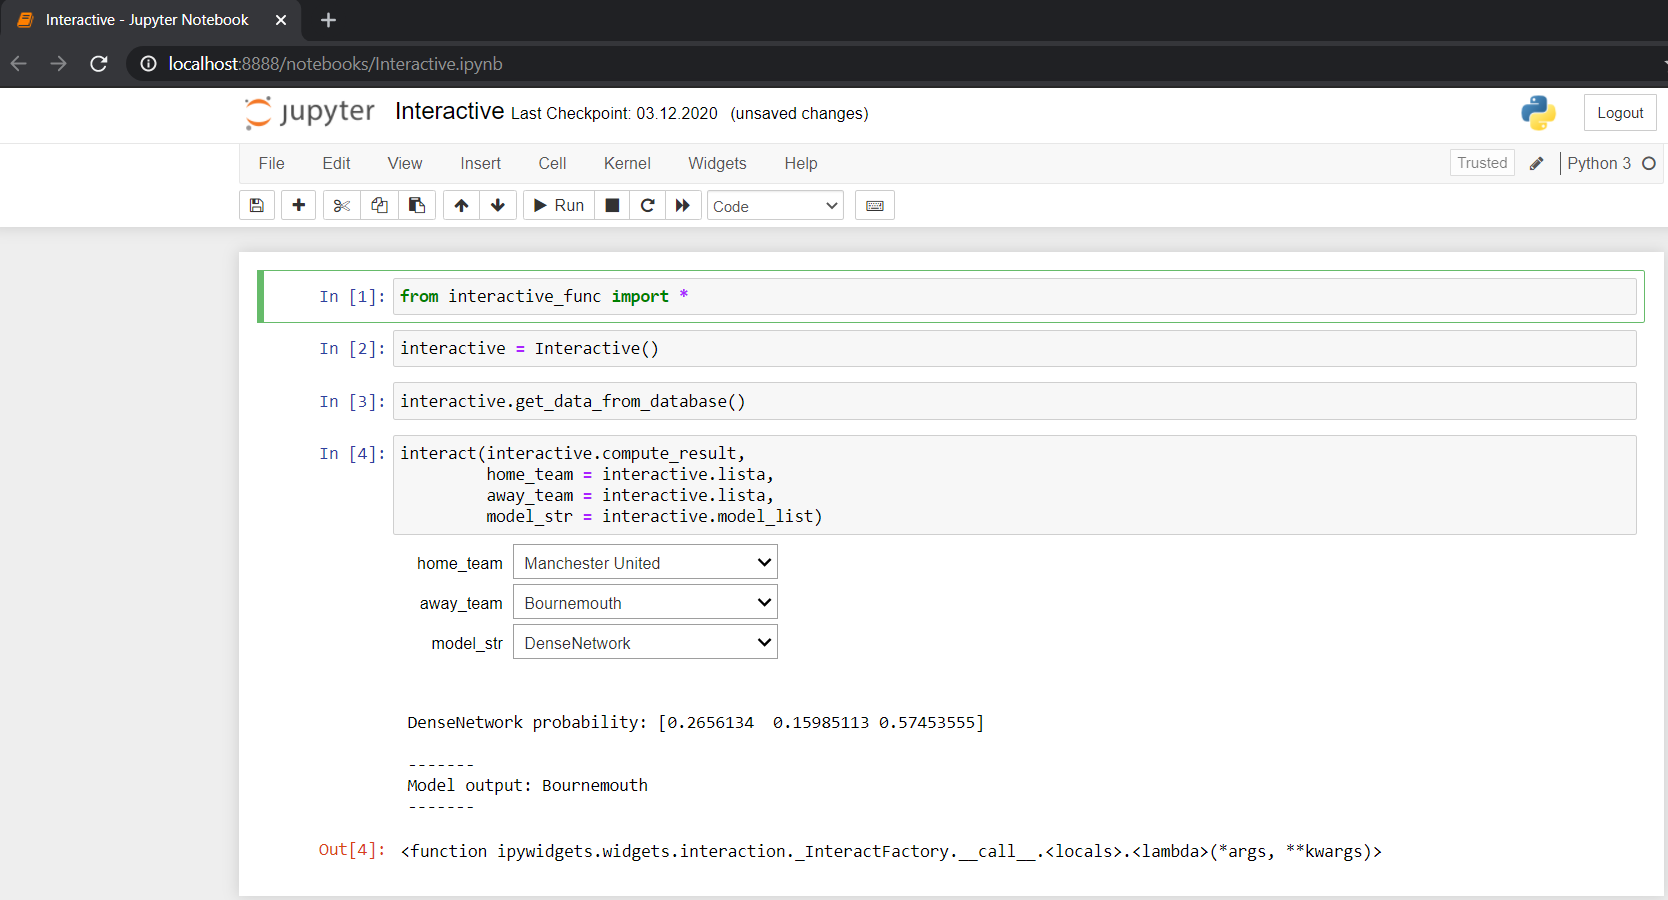
\includegraphics[width=16cm,height=10cm]{figures/Interactive_overview.png}
        \caption{Interaktywny notebook}\label{interactive}
\end{figure}
Do uruchomienia środowiska potrzebne jest uruchomienie czterech przedstawionych powyżej komórek programu, a funkcje, które zostaną dzięki temu wykonane, zadbają o to by użytkownik mógł bez pisania jakiegokolwiek kodu pobrać wymagane dane a następnie dokonać predykcji.

Wybór drużyn odbywa się poprzez wybór z rozwijanego menu:
\begin{figure}[H] 
        \centering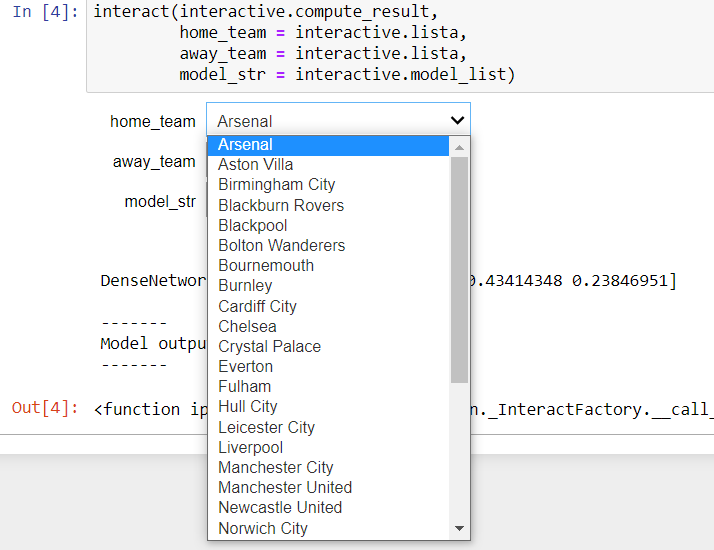
\includegraphics[width=10cm,height=8cm]{figures/Interactive_team_selection.png}
        \caption{Interaktywny wybór drużyn}\label{interactive_tem}
\end{figure}
Dodatkowo, pozwala się użytkownikowi na wybór preferowanego przez niego algorytmu, za pomocą którego zwrócony zostanie wynik predykcji:
\begin{figure}[H] 
        \centering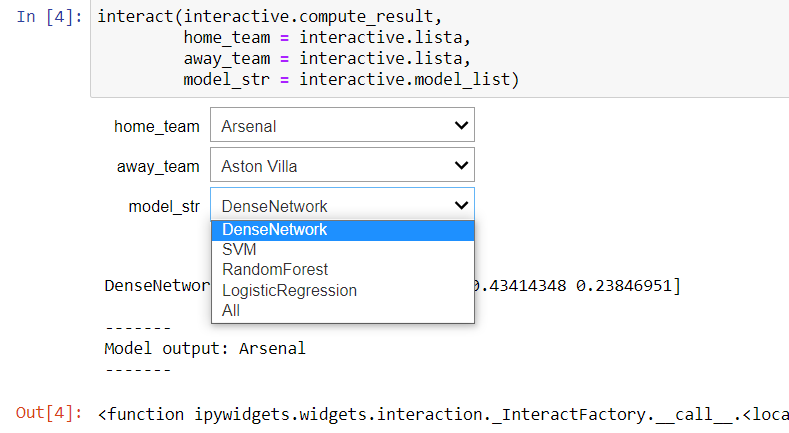
\includegraphics[width=12cm,height=8cm]{figures/Interactive_alg_selection.png}
        \caption{Interaktywny wybór algorytmu}\label{interactive_alg}
\end{figure}
W momencie, kiedy użytkownik wyraziłby chęć wykorzystania wszystkich algorytmów, zostaje mu udostępniona taka możliwość i na zasadzie głosowania większościowego (klasa, które uzyska większość głosów zostaje zwrócona, w przeciwnym wypadku komunikat od braku dominanta i zachęcenia do wybrania konkretnego algorytmu) użytkownik jest wstanie uzyskać wynik. W przypadku algorytmów, które zwracają rozkład prawdopodobieństwa przynależności do konkretnych klas wynikowych, również ta informacja jest zwrócona i wyświetlona dla użytkownika, w celu pokazania mu czy dany wynik jest bardziej lub mniej pewny według wybranego algorytmu. 

\begin{figure}[H]%
    \centering
    \subfloat[\centering Wynik wraz z prawdopodobieństwem]{{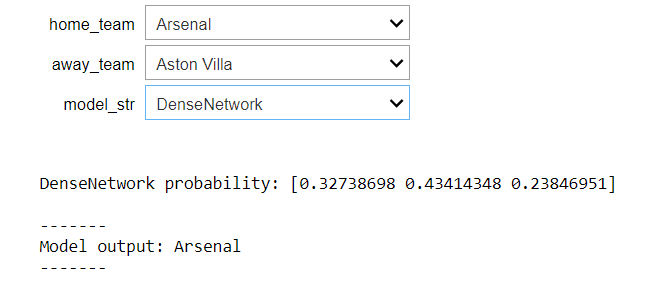
\includegraphics[width=6cm,height=5cm]{figures/Interactive_results.png} }}%
    \qquad
    \subfloat[\centering Brak wyniku dominującego]{{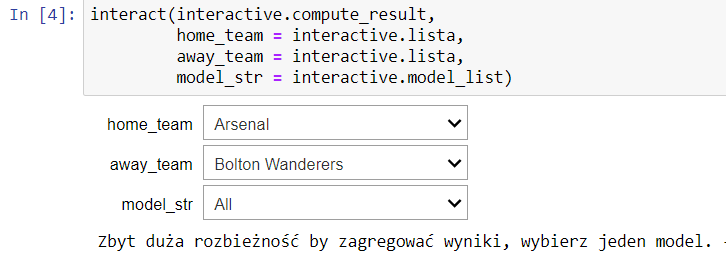
\includegraphics[width=8cm,height=5cm]{figures/Interactive_results2.png} }}%
    \caption{Otrzymywane odpowiedzi zwrotne}%
    \label{fig:Results}%
\end{figure}
Podsumowując, interaktywny notebook jest bardzo prostym lecz zarazem intuicyjnym interfejsem, który każdy może z powodzeniem wykorzystać i odczytać wyniki na podstawie nauczonych modeli predykcyjnych.
\chapter{Własne propozycje rozwiązań}
    \section{Pozyskanie i agregowanie danych}
        \subsection{Europejska baza danych piłkarskich}
        \subsection{Elo Rating klubów piłkarskich}
        \subsection{Historyczne dane zakładów piłkarskich}
        \subsection{Metody agregacji}
    \section{Web API}
    \section{Wizualizacja charakterystyk danych}
    \section{Wstępne przetwarzanie}
        \subsection{Pobieranie danych z serwera}
        \subsection{Tworzenie zbioru cech}
        Zbiór cech jest jednym z kluczowych czynników, które wpływają na jakość algorytmów uczenia maszynowego. Odpowiedni dobór oraz selekcja i segregacja to dobra drogo do uzyskania dobrej predykcji. Jednak wybór odpowiednich cech nie jest łatwym zadaniem i zazwyczaj zajmuje on dużo czasu i zasobów. Także w naszym problemie, dobór cech był starannie dokonany. Piłka nożna do bardzo rozbudowana gra i z jednej partii między drużynami można wyciągnąć nieskończoną ilość danych, poprzez najbardziej oczywiste jak liczba strzałów, po te mniej jak ilość minut spędzonych na swojej połowie przez danego gracza lub średni wiek piłkarza w danej drużynie. Z racji, że posiadaliśmy dość rozbudowaną bazę pochodzącą z różnych źródeł, ostatecznie wybraliśmy 30 cech, które odpowiednio zagregowaliśmy a następnie przekazaliśmy na wejście naszych algorytmów uczenia maszynowego. Lista tych cech wraz z ich krótkim wyjaśnieniem: .
        
        \begin{itemize}
            \item avg\_away\_win\_odds, avg\_home\_win\_odds, avg\_draw\_odds: średnia wartość kursów oferowanych na zwycięstwo danej drużyny, remis oraz wygraną drugiej drużyny,
            \item home\_elo\_rating, away\_elo\_rating: ELO rating dla obu drużyn,
            \item home\_players\_avg\_age, away\_players\_avg\_age: średni wiek graczy w drużynach, 
            \item home\_players\_avg\_rating, away\_players\_avg\_rating: zagregowana siła zawodników danej drużyny (statystyki z gry Fifa takie jak: drybling, kontrola piłki, strzały z daleka ...), 
            \item home\_team\_score, away\_team\_score: siła drużyny (statystyki z gry Fifa takie jak: szybkość, budowania ataku, ilość wymienianych podań ...), 
            \item home\_avg\_corners, away\_avg\_corners: średnia liczba rzutów rożnych na mecz danej drużyny w ciągu ostatnich 3 meczów, 
            \item home\_avg\_shots, away\_avg\_shots: średnia liczba oddanych strzałów na mecz danej drużyny w ciągu ostatnich 3 meczów, 
            \item home\_won\_games, away\_won\_games: liczba wygranych przez drużynę spotkań z ostatnich 3 meczów, 
            \item home\_tied\_games, away\_tied\_games: liczba remisów w ostatnich 3 meczach, 
            \item home\_lost\_games, away\_lost\_games: liczba przegranych w ostatnich 3 meczach, 
            \item home\_scored\_goals, away\_scored\_goals: liczba strzelonych przez drużynę goli w ostatnich 3 meczach, 
            \item home\_team\_last\_season\_points, away\_team\_last\_season\_ponits: zdobyte punkty przez drużynę w ostatnim sezonie, 
            \item home\_team\_seasons\_played, away\_team\_seasons\_played: liczba sezonów, które dana drużyna gra w Premier League, 
            \item home\_direct\_wins: liczba zwycięstw drużyny gospodarza nad drużyną gościa w ostatnich meczach rozgrywanych przeciwko sobie,
            \item away\_direct\_wins: liczba zwycięstw drużyny gościa nad drużyną gospodarza w ostatnich meczach rozgrywanych przeciwko sobie, 
            \item direct\_draws: liczba remisów drużyny gościa z drużyną gospodarzy w ostatnich meczach rozgrywanych przeciwko sobie. 


        \end{itemize}   
        
        \subsection{Agregacja danych}
        \subsection{Testowanie jednostkowe}
    \section{Algorytmy}
    Po przetworzeniu danych i ich przygotowaniu kolejnym krokiem w realizacji naszego projektu jest dostosowanie wydajnych algorytmów. W tej sekcji zaprezentujemy własne rozwiązania dla postawionego przez nas zadania. Przedstawimy kolejno cztery algorytmy, które wypróbowaliśmy i dały rzetelne rezultaty. Pokażemy ich strukturę oraz parametry dobrane w taki sposób by maksymalizować jakość naszego rozwiązania oraz osiągane wyniki.
        \subsection{Sztuczna Sieć Neuronowa - SNN}
        Pierwszym podejściem, które zaprezentujemy jest zbudowana przez nas na potrzeby zadania sztuczna sieć neuronowa. Przechodząc do budowy sieci, która zastosowaliśmy możemy ją opisać jako jednokierunkowa, sekwencyjna sieć posiadająca dwie warstwy ukryte, warstwę wejściową i wyjściową. Po każdej warstwie poza wyjściową, użyta jest warstwa normalizacji wsadowej (\english{BatchNormalization}) \cite{BatchNormalization}. Dodatkowo po pierwszej (i tylko po niej) zastosowaliśmy technikę Monte Carlo wraz z losowym porzucaniem połączeń pomiędzy neuronami (\english{Monte Carlo (MC) Dropout}) \cite{MCDropout} \cite{Dropout} \cite{Dropout2}. W pierwszej warstwie, warstwie wejściowej zastosowaliśmy 40 neuronów, które przepuszczją swoją kombinację danych wejściowych przez funkcję aktywacji \definicja{relu}: \[ReLU(x) = max(0, x)\] co sprawia, że funkcja na wyjściu przekazuje wartości nieujemne. Kolejno w warstwie \definicja{MCDropout} ustawiliśmy współczynnik porzucania równy 0.3. Następna warstwa ukryta składała się z 40 neuronów i funkcji aktywacji \definicja{selu} \cite{SELU} a jej formuła ma się następująco:
        \[
        SELU(x) = \lambda
        \begin{cases}
            x &  \text{if}\ x > 0\\
            \alpha e^{x} - \alpha &  \text{if}\ x \le 0
        \end{cases}
        \]
        gdzie:
        \begin{center}
            $\alpha \approx 1.6732632423543772848170429916717$ \\ 
            $\lambda \approx 1.0507009873554804934193349852946$
        \end{center}
        Następnie w warstwie ukrytej również zastosowaliśmy funkcję aktywacji \definicja{selu}, lecz tym razem umieściliśmy zaledwie 5 neuronów. Wasrtwa wyjściowa składała się z ilości neuronów odpowiadającej ilości klas równej 3 (Draw, HomeWin, AwayWin), a funkcja aktywacji to funkcja \definicja{softmax}:
        \[
        \hat{p}_{k} = \sigma(s(x))_{k} = \frac{exp \big(s_{k}(x)\big)}{\sum_{j=1}^{K}exp \big(s_{j}(x)\big)}
        \]
        gdzie:
        \begin{itemize}
            \item K to liczba klas,
            \item s(x) to wektor zawierający wyniki każdej klasy dla instancji x,
            \item $\sigma(s(x))_{k}$ jest szacowanym prawdopodobieństwem, że instancja x należy do klasy k, biorąc pod uwagę wyniki każdej klasy dla tej instancji.
        \end{itemize}
        Model sekwencyjny uczyliśmy przy pomocy optymalizatora \definicja{nadam} \cite{adam} \cite{nadam} wraz z funkcją straty \definicja{sparse categorical corossentropy}. Wstępnie ustawiliśmy 80 epok, które miały za zadanie uzyskać najlepszy wynik dla naszego problemu, jednak wczesne zatrzymywanie (\english{early stopping}) pozwoliło na zatrzymanie treningu już na dwudziestej pierwszej epoce chroniąc nasz model przed przeuczeniem (\english{overfitting}).
        
        Po treningu, w celu testowania i predykcji wyników, zastosowana warstwa \definicja{MCDropout} pozwala na kontynuowanie porzucania nawet w fazie po treningowej (w przeciwieństwie do podstawowej techniki \definicja{Dropout}, która po nauczeniu sieci, w fazie testowania nie porzucała neuronów - nie spełniała już żadnej funkcji) i dzięki temu zastosowaliśmy technikę, w której nowy przykład, którego klasę chcemy przewidzieć, jest przepuszczany przez sieć 100 razy, każdy wynik z poszczególnego przebiegu jest przechowywany, a następnie uśredniany dla każdej z możliwych klas. Po tej operacji posiadaliśmy bardziej rzetelne wyniki, które przełożyły się na lepsze rezultaty na zbiorze testowym.
        
        Schemat sieci można przedstawić w postaci tabeli \ref{tab:SNNTable}
        \begin{table}[H]
            \centering
            \caption{Schemat SNN}
            \label{tab:SNNTable}
            \begin{tabular}{|c|c|c|}
            \hline
                Layer (type) &  Output Shape & Param \#\\ \hline \hline
                dense (Dense) & (None, 40) & 1240 \\ \hline
                batch\_normalization (BatchNormalization) & (None, 40) & 160 \\ \hline 
                mc\_dropout (MCDropout) & (None, 40) & 0 \\ \hline         
                dense\_1 (Dense) & (None, 40) & 1640 \\ \hline      
                batch\_normalization\_1 (BatchNormalization) & (None, 40) & 160 \\ \hline
                dense\_2 (Dense) & (None, 5) &  205 \\ \hline       
                batch\_normalization\_2 (BatchNormalization)  & (None, 5) &  20 \\ \hline
                dense\_3 (Dense) & (None, 3) &  18 \\ \hline \hline 
            \end{tabular}
            	\begin{tabular} {| c |}
                Total params: 3,443 \\
                Trainable params: 3,273 \\
                Non-trainable params: 170 \\
                \hline
                \end{tabular}
        \end{table}
        \subsection{SVM}
        Kolejnym podejściem, które braliśmy pod uwagę i testowaliśmy, był algorytm \definicja{SVM}. W podejściu tym skupiliśmy się na znalezieniu trzech najlepszych parametrów (C, $\gamma$, jądro (\english{kernel})). W celu znalezienia tych parametrów, zastosowaliśmy technikę losowego przeszukiwania siatki (\english{Randomized Search CV}) \cite{SKcv}, której jako punkt odniesienia zaaplikowaliśmy metrykę \definicja{f1\_macro} \cite{SKf1}. Zbiór walidacyjny potrzebny do szacowania wyników oraz porównywania dobranych parametrów podczas szukania, został przedstawiony w sekcji \ref{section:ocenaWynikow} i dotyczył on dzielenia zbioru danych na następujące po sobie bloki.
        
        Po fazie przeszukiwania, wybrane zostały najlepsze parametry, które przedstawiają się następująco:
        \begin{table}[H]
            \centering
             \caption{Parametry SVM}
            \label{tab:my_label}
            \begin{tabular}{| c c |}
            \hline
                 Parametr & wartość \\ \hline \hline
                 C & 3.560291686892903 \\ \hline
                 $\gamma$ & 0.0030492848805430566 \\ \hline
                 jądro & rbf \\ \hline
            \end{tabular}
        \end{table}
        \subsection{Alg3}
        \subsection{Alg4}
\chapter{Wyniki oceny eksperymentalnej}

\noindent W tej sekcji zostaną przedstawione oceny predykcji wyników meczy piłkarskich osiągnięte na danych testowych przez wybrane algorytmy uczące się wchodzące w skład systemu. 

Chcemy przypomnieć, że sport, jakim jest piłka nożna, należy do dyscyplin bardzo złożonych, charakteryzujących się ogromną liczbą zmiennych, które są słabo przewidywalne i trudne do uwzględnienia. Ponadto w rzeczywistości wynik predykcji meczu  determinowany jest pewną dozą szczęścia dla jednej z drużyn. Inne czynniki są również trudne do uwzględnienia. Warunki pogodowe, dyspozycja danego zawodnika oraz nastawienie każdego z graczy jest często czynnikiem kluczowym, lecz niestety niemożliwym do uchwycenia w przypadku typowych danych historycznych, a tym bardziej w celu wykorzystania do predykcji wyniku spotkania. Jednak istnieją również czynniki reprezentowane przez atrybuty, które mają realny wpływ na wynik i właśnie je postarano się w tej pracy zidentyfikować, uwzględnić oraz na ich podstawie dokonywać obliczeń i zwracać rezultaty o potencjalnym zwycięzcy. Dane przygotowane i przetworzone (patrz opis w poprzednich rozdziałach) były podstawą do osiągnięcia wyników naszego systemu, które przedstawiono w poszczególnych podsekcjach dla wybranych algorytmów. 

W posiadanych danych występują 3 następujące klasy, które trzeba przewidzieć: 
\begin{itemize}
    \item \english{Draw} - oznacza remis pomiędzy drużynami (etykieta 0)
    \item \english{HomeWin} - oznacza, że drużyna definiowana jako gospodarz odniosła zwycięstwo (etykieta 1)
    \item \english{AwayWin} - oznacza, że drużyna definiowana jako gość odniosła zwycięstwo (etykieta 2)
\end{itemize}

Liczba przykładów z poszczególnych klas w zbiorze danych przed operacją odlosowania przedstawiono w tabeli \ref{tab:przedOdlosowaniem} 

\begin{table}[H]
    \centering
    \caption{Liczba przykładów  w poszczególnych klasach przed odlosowaniem}
    \label{tab:przedOdlosowaniem}
    \begin{tabular}{| c  c |}
    \hline
         Draw & 586 \\
         HomeWin & 1021 \\
         AwayWin & 662 \\\hline
    \end{tabular}
\end{table}
Jak widać, klasa oznaczająca wygraną drużyny gospodarzy, posiada prawie dwukrotnie więcej przykładów niż pozostałe klasy. Dlatego powyższy zbiór danych został zmniejszony w taki sposób, że najliczniejsza klasa została w przybliżeniu wyrównana do klasy mniej licznej uzyskując w ten sposób bardziej zbalansowane dane, w których nie ma jednej, bardzo dominującej klasy. Metoda wykorzystana do zmniejszenia danych to losowe usunięcie elementów z klasy najbardziej licznej (odpowiednik metod z grupy \english{undersampling}) i właśnie taki zbiór został wykorzystany w dalszym etapie algorytmów (wyniki operacji można zaobserwować w tabeli \ref{tab:poOdlosowaniu}). 

\begin{table}[H]
    \centering
    \caption{Liczba przykładów w poszczególnych klasach po odlosowaniu}
    \label{tab:poOdlosowaniu}
    \begin{tabular}{| c  c |}
    \hline
         Draw & 586 \\
         HomeWin & 662 \\
         AwayWin & 662 \\\hline
    \end{tabular}
\end{table}
Kolejnym krokiem było przygotowanie odpowiednich zbiorów (testowy, walidacyjny oraz treningowy) i rozkład poszczególnych klas w tych zbiorach można zobaczyć w tabeli \ref{tab:rozkłądDanych}.

\begin{table}[H]
\caption{Rozkład danych w odpowiednich zbiorach}
\label{tab:rozkłądDanych}
\centering
\begin{tabular}{| c | c c c |}
\hline
    Klasa & zbiór treningowy & zbiór walidacyjny & zbiór testowy \\ \hline
   Draw & 489 & 32 & 65 \\
   HomeWin & 572 & 31 & 59  \\
   AwayWin & 562 & 33 & 67 \\ \hline
\end{tabular}
\end{table}


We wszystkich algorytmach próbowano również sposobu na nadlosowanie przykładów uczących metodą GlobalCS \cite{GlobalCS} i niestety w każdym z algorytmów rezultaty na wartości trafności (\english{accuracy}) były niższe, dlatego zrezygnowano z tej techniki.

\section{Sztuczne sieci neuronowe}
\label{SNN-results}
\noindent W tej podsekcji, przedstawione zostaną wyniki, które udało się osiągnąć dla struktury sztucznej sieci neuronowej, której parametry wraz z opisem zostały przedstawione w sekcji \ref{SNN-opis} oraz \ref{SNN-param}. Ogólna dokładność - trafność predykcji (\english{accuracy}), obliczona na zbiorze testowym, stanowiącym 10\% z dostępnego zbioru danych wyniosła \definicja{50.79\%}, co w ogólności jest wynikiem satysfakcjonującym, ponieważ w chwili w której osoba zainteresowana predykcją zgadywała by wynik spotkania z równym prawdopodobieństwem wystąpienia jednego z trzech rezultatów, średnia trafność wyniosłaby około 33\%, tak więc wartość powyżej tej liczby jest czymś więcej niż opcją zwykłego zgadywania wyniku. Ponadto inne algorytmy nie doprowadzały do dokładności radykalnie wyższych. 

Wartości innych miar przedstawiono w tabeli \ref{tab:SNNscore}.

\begin{table}[H]
    \centering
    \caption{Wyliczone średnie wartości miar klasyfikacyjnych dla SNN}
    \label{tab:SNNscore}
    \begin{tabular}{| c | c |}
    \hline
         Precyzja (\english{precision}) &  50.41\%\\
         \hline
         Czułość (\english{recall}) &  51.06\%\\
         \hline
         Wartość Fscore &  49.78\%\\
         \hline
    \end{tabular}
\end{table}


Przypomnijmy że miarę precyzji można interpretować jako stosunek $\frac{tp}{tp + fp}$, gdzie tp to liczba poprawnie sklasyfikowanych przykładów, a fp to liczba niepoprawnie sklasyfikowanych przykładów negatywnych jako klasy pozytywnej. Czułość z kolei można interpretować jako stosunek $\frac{tp}{tp + fn}$, gdzie tp jest liczbą poprawnie sklasyfikowanych przykładów pozytywnych, a fn liczba niepoprawnie sklasyfikowanych przykładów pozytywnych jako predykcji w klasie negatywnej -- czyli jest to lokalna dokładność rozpoznania klasy. Fscore interpretuje się jako ważoną średnią harmoniczną precyzji i czułości. Dodatkowo, warto zaznaczyć, że miary te są obliczane na podstawie nieważonej średniej poszczególnych wyników z tych miar i właśnie dlatego, tabela \ref{tab:SNNscore} zawiera pojedyncze wartości takich średnich po klasach. 
Macierz pomyłek przedstawia się następująco:

\begin{center}
\begin{table}[H]
\renewcommand{\arraystretch}{1.5}
\caption{Macierz pomyłek dla SNN}
\label{tab:macierzSNN}
\begin{center}
\begin{tabular}{|c|c|c|c|c|}
   \cline{3-5} 
   \multicolumn{1}{c}{} & & \multicolumn{3}{c|}{Predicted} \\ \cline{3-5}
   \multicolumn{1}{c}{} & & Draw & HomeWin & AwayWin \\ \hline
   
   {Observed/actual}
   & Draw & 20 & 23 & 22 \\ \cline{2-5}
   & HomeWin & 12 & 37 & 10  \\ \cline{2-5}
   & AwayWin & 10 & 17 & 40 \\ \hline
\end{tabular}
\end{center}
\end{table}
\end{center}


Można zauważyć, że najwięcej błędów popełnianych w predykcji, jest w momencie, kiedy faktyczna klasa symbolizuje remis pomiędzy drużynami. 

Po procesie nauki sieci postanowiono dodatkowo sprawdzić wpływ danych cech wejściowych na predykcję danego wyniku i odkryć, które atrybuty odgrywały kluczowe role dla predykcji konkretnego wyniku. Dokonaliśmy tego przy użyciu wartości Shapleya \cite{shapley} oraz biblioteki w języku Python \definicja{Shap}.
\begin{figure}[H] 
        \centering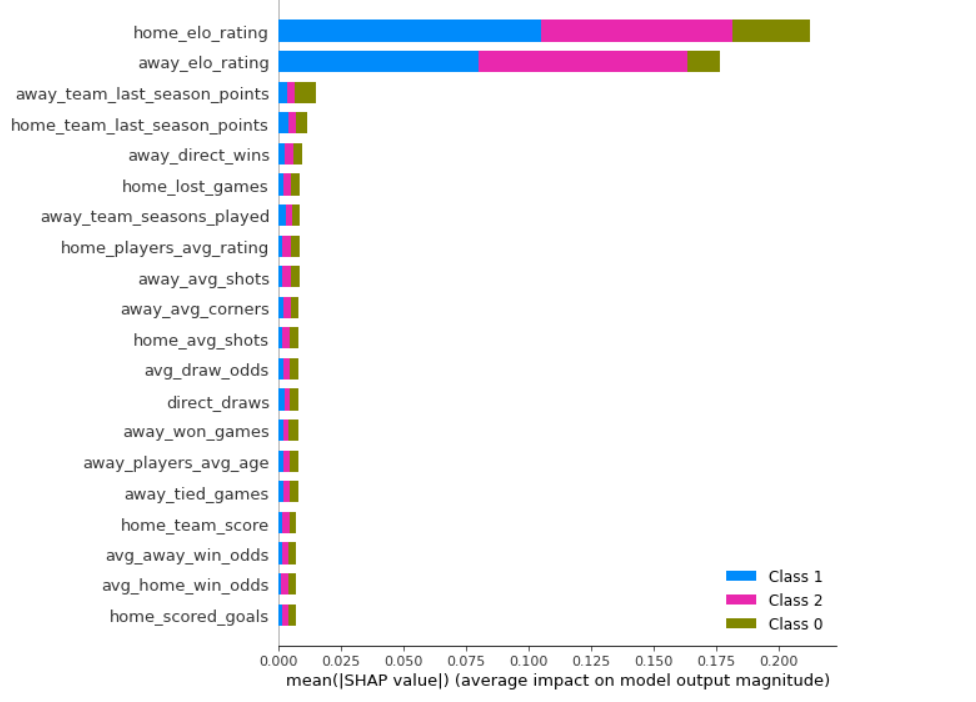
\includegraphics[width=10cm,height=6cm]{figures/ShapSNN.png}
        \caption{Wartości Shapleya dla SNN}\label{Shap-SNN}
\end{figure}

Jak można zauważyć na rysunku \ref{Shap-SNN}, atrybut \textit{home\_elo\_rating} oraz \textit{away\_elo\_rating} miały największe znaczenie (wartość Shapleya), które w największym stopniu wpływa na wyniki predykcji sieci. Nie jest to zaskakujący rezultat, ponieważ atrybut ten jest odzwierciedleniem ogólnej siły drużyny w danym meczu oraz aktualizowany jest co spotkanie więc można było się spodziewać dużego znaczenia tej cechy. Ponadto jego przydatność wskazywano w przeglądanej literaturze o analizie rozgrywek piłkarskich. Dodatkowo, warto zauważyć, że cecha określająca liczbę punktów w zeszłych sezonach danej drużyny również była uznana za mocno wpływającą na predykcje (choć  mniej niż wartości atrybutu elo\_rating) i można ją zinterpretować jako dotychczasowy sposób radzenia sobie danej drużyny w analizowanej lidze.

\section{Metoda wektorów wspierających}
\noindent Ta sekcja będzie prezentować wyniki dla algorytmu SVM. Dokładność (\english{accuracy}) na  zbiorze testowym (takim samym jak poprzednio) wyniosła 49.74\%. Dodatkowe miary, które interpretuje się również tak samo jak w podsekcji \ref{SNN-results}, wyglądają następująco:

\begin{table}[H]
    \centering
    \caption{Wyliczone średnie wartości miar dla SVM}
    \label{tab:SVMscore}
    \begin{tabular}{| c | c |}
    \hline
         Precyzja (\english{precision}) &  48.79\%\\
         \hline
         Czułość (\english{recall}) &  49.90\%\\
         \hline
         Wartość Fscore &  48.45\%\\
         \hline
    \end{tabular}
\end{table}
Dodatkowo, macierz pomyłek została przedstawiona w tabeli \ref{tab:macierzSVM}
\begin{center}
\begin{table}[H]
\renewcommand{\arraystretch}{1.5}
\caption{Macierz pomyłek dla SVM}
\label{tab:macierzSVM}
\begin{center}
\begin{tabular}{|c|c|c|c|c|}
   \cline{3-5} 
   \multicolumn{1}{c}{} & & \multicolumn{3}{c|}{Predicted} \\ \cline{3-5}
   \multicolumn{1}{c}{} & & Draw & HomeWin & AwayWin \\ \hline
   
   {Observed/actual}
   & Draw & 18 & 21 & 26 \\ \cline{2-5}
   & HomeWin & 13 & 35 & 11  \\ \cline{2-5}
   & AwayWin & 10 & 15 & 42 \\ \hline
\end{tabular}
\end{center}
\end{table}
\end{center}
Również przy użycia tego klasyfikatora, prawidłowa predykcja remisu jest najsłabsza. Predykcja zwycięstw oraz porażek jest dużo bardziej skuteczna.

Również dalej wykorzystano wartości Shapleya \cite{shapley} z użyciem  biblioteki w języku Python \definicja{Shap}  w celu określenia, które kombinacje cech miały największy wpływ na otrzymywany wynik w naszym algorytmie.

\begin{figure}[H] 
        \centering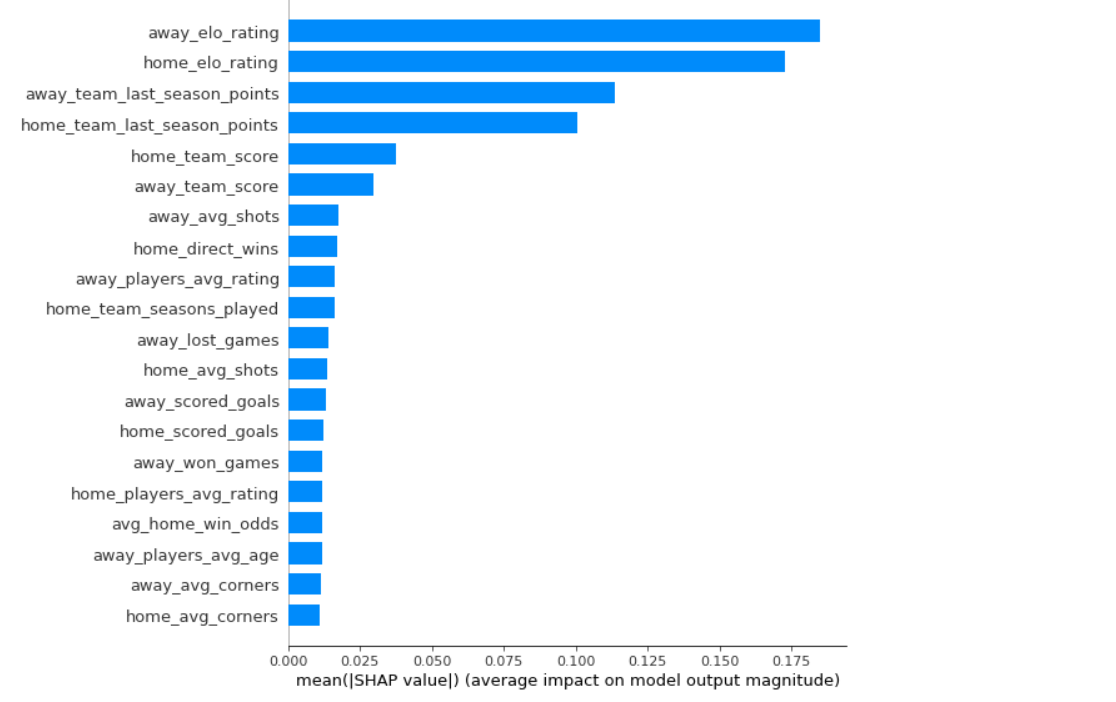
\includegraphics[width=10cm,height=6cm]{figures/ShapSVM.png}
        \caption{Wartości Shapleya dla SVM}\label{Shap-SVM}
\end{figure}
W tym przypadku, również wartości elo\_rating odgrywały kluczową rolę dla algorytmu SVM. Interpretacja może być podobna, gdyż wartość ta to zagregowana i wyliczona wartości siły i zdolności danej drużyny, czyli mająca realny wpływ na to, jak dana drużyna ma aktualnie predyspozycje oraz zdolności. Ponadto wysoką wartość przyjęły atrybuty takie jak liczba punktów danych drużyn w poprzednim sezonie oraz liczba punktów danej drużyny w aktualnie rozgrywanym sezonie. 

%Wszystkie te czynniki, oraz dobór parametrów dały rezultaty jak przedstawiono powyżej.

\section{Regresja logistyczna}
\noindent W tej sekcji przedstawione zostaną wyniki osiągnięte przez algorytm regresji logistycznej z parametrami modelu opisanymi szczegółowo w sekcji \ref{tab:params_lr}.

Testy dla algorytmu regresji logistycznej zostały przeprowadzone na kilku wersji zbiorów danych. Oprócz  oryginalnych zbiorów, rozważono pomniejszone zbiory (jak w poprzednich testach), w których pomniejszenie polegało na losowym usunięciu przykładów z klasy najbardziej licznej (\english{undersampling}). Spróbowano także wykorzystać nadlosowanie przykładów uczących metodą GlobalCS w ten sposób, że liczba obserwacji z klas najmniej licznych została wyrównana do liczby obserwacji z klasy najbardziej licznej (\english{oversampling}). Dla każdej z tej metod nauczono od podstaw algorytm klasyfikujący oraz przeprowadzono predykcję na zbiorze testowym (liczność zbioru testowego wyniosła 10\% obserwacji całego zbioru danych).

\begin{table}[H]
    \centering
    \caption{Wyliczone średnie wartości miar w różnych podejściach dla danych niezbalansowanych dla algorytmu regresji logistycznej}
    \label{tab:LRSampling}
    \begin{tabular}{| c | c | c | c | c |}
    \hline
        Podejście & Dokładność & Prezycja & Czułość & Wartość Fscore \\ \hline 
        \hline
        Oryginalny zbiór danych & 46.7\% & 44.06\% & 45.32\% & 43.95\% \\
        \hline
        \textit{Undersampling} & 52.88\% & 52.21\% & 53.16\% & 52.3\% \\
        \hline
        \textit{GlobalCS} & 45.81\% & 42.75\% & 42.74\% & 42.18\% \\
         \hline
    \end{tabular}
\end{table}

Analizując wyniki otrzymane poprzez wykorzystanie różnych podejść do problemu niezbalansowanych danych można stwierdzić, że dla algorytmu regresji logistycznej zdecydowanie najlepiej sprawdza się metoda polegająca na usunięciu obserwacji z klas bardziej licznych, która jest wykorzystana także w innych podrozdziałach.

Ponadto wykonany został kolejny test sprawdzający ile meczów wstecz dla danej drużyny powinniśmy brać pod uwagę przy wyliczaniu cech dla naszego algorytmu, tak aby maksymalizować średnie wartości dokładności, precyzji oraz czułości.

\begin{table}[H]
    \centering
    \caption{Znalezienie odpowiedniej liczby meczów dla wyliczanych cech w algorytmie regresji logistycznej}
    \begin{tabular}{| c | c | c | c | c |}
    \hline
        Liczba meczów wstecz & Dokładność & Prezycja & Czułość & Wartość Fscore \\ \hline 
        \hline
        Trzy mecze wstecz & 52.88\% & 52.21\% & 53.16\% & 52.3\% \\
        \hline
        Cztery mecze wstecz & 51.31\% & 50.97\% & 51.43\% & 50.98\% \\
        \hline
        Pięć meczów wstecz & 52.36\% & 51.71\% & 52.53\% & 51.77\% \\
         \hline
    \end{tabular}
\end{table}

Przyglądając się wynikom osiągniętym w powyższej tabeli dla dalszych testów algorytmu wykorzystany został zbiór danych, dla którego odpowiednie statystyki wyliczone są na podstawie trzech meczów wstecz.

Dokonano także przeglądu cech wykorzystywanych w algorytmie, po której to analizie zdecydowano się usunąć ze zbioru treningowego jak i uczącego cechy: \textit{home\_direct\_wins}, \textit{away\_direct\_wins}, \textit{direct\_draws}, gdyż cechy te nie dostarczały istotnych informacji algorytmowi oraz wpływały negatywnie na osiągane przez niego rezultaty. Po powyższej redukcji dokładność klasyfikacji na zbiorze testowym wyniosła 53.40\%. Poszczególne średnie wartości miary precyzji, czułości oraz wartości Fscore prezentują się następująco:

\begin{table}[H]
    \centering
    \caption{Wyliczone średnie wartości miar dla algorytmu regresji logistycznej}
    \label{tab:LRscore}
    \begin{tabular}{| c | c |}
    \hline
         Precyzja (\english{precision}) &  52.81\%\\
         \hline
         Czułość (\english{recall}) &  53.80\%\\
         \hline
         Wartość Fscore &  52.79\%\\
         \hline
    \end{tabular}
\end{table}

\newpage

Macierz pomyłek dla tego algorytmu prezentuje się następująco:

\begin{center}
\begin{table}[H]
\renewcommand{\arraystretch}{1.5}
\caption{Macierz pomyłek dla algorytmu regresji logistycznej}
\begin{center}
\begin{tabular}{|c|c|c|c|c|}
   \cline{3-5} 
   \multicolumn{1}{c}{} & & \multicolumn{3}{c|}{Predicted} \\ \cline{3-5}
   \multicolumn{1}{c}{} & & Draw & HomeWin & AwayWin \\ \hline
   
   {Observed/actual}
   & Draw & 23 & 18 & 24 \\ \cline{2-5}
   & HomeWin & 10 & 40 & 9  \\ \cline{2-5}
   & AwayWin & 15 & 13 & 39 \\ \hline
\end{tabular}
\end{center}
\end{table}
\end{center}

Na podstawie powyższych wyników można wyciągnąć podobne wnioski jak we dwóch wcześniejszych podejściach. Algorytm zdecydowanie radził sobie najgorzej z typowaniem remisów w przeciwieństwie do typowania zwycięstwa którejś z drużyn. \\

Ważność odpowiednich cech dla algorytmu została ustalona poprzez wykorzystanie metody \textit{coef\_} dla modelu regresji logistycznej z biblioteki \textit{scikit-learn}. Wartości z poniższej tabeli należy odpowiednio interpretować: im wyższa wartość współczynnika dla danej cechy tym ta cecha odgrywała większą rolę w procesie predykcji ostatecznej klasy dla danej obserwacji. Analogicznie im mniejsza wartość współczynnika tym ważność danej cechy w całym procesie była mniejsza. Tabela zbierająca ważności cech prezentuje się następująco:

\begin{table}[H]
        \caption{Ważność cech modelu regresji logistycznej}
        \centering
        \begin{tabular}{c c c}
        \toprule
            Cecha & Współczynnik \\
        \midrule
            avg\_away\_win\_odds & 0.0232 \\
            home\_avg\_shots & 0.0215 \\
            avg\_home\_win\_odds & 0.0203 \\
            home\_scored\_goals & 0.0198 \\
            away\_avg\_shots & 0.0166 \\
            away\_players\_avg\_age & 0.016 \\
            home\_players\_avg\_rating & 0.0159 \\
            away\_players\_avg\_rating & 0.0148 \\
            home\_team\_seasons\_played & 0.0147 \\
            away\_won\_games & 0.0108 \\
            away\_avg\_corners & 0.0105 \\
            avg\_draw\_odds & 0.0097 \\
            home\_avg\_corners & 0.0077 \\
            away\_lost\_games & 0.0073 \\
            away\_tied\_games & 0.0064 \\
            away\_scored\_goals & 0.0063 \\
            home\_tied\_games & 0.0039 \\
            away\_team\_score & 0.0039 \\
            home\_players\_avg\_age & 0.0038 \\
            away\_team\_seasons\_played & 0.0034 \\
            home\_team\_score & 0.0033 \\
            away\_team\_last\_season\_points & 0.0021 \\
            home\_lost\_games & 0.0019 \\
            home\_elo\_rating & 0.0019 \\
            away\_elo\_rating & 0.0014 \\
            home\_team\_last\_season\_points & 0.0009 \\
            home\_won\_games & 0.0008 \\
        \bottomrule
        \end{tabular}
        \end{table}

Na podstawie powyższej tabeli można zauważyć, że najwyższy wpływ na dokonaną predykcję mają wartości kursów oferowanych przez zakłady bukmacherskie. Zdawano sobie sprawę, że te atrybuty mogą mieć znaczenie w problemie predykcji wyniku meczu, dlatego nie jest to rezultat zaskakujący. Warto także podkreślić wartości dla cech związanych z liczbą strzałów oraz liczbą zdobytych goli w ostatnich meczach. W przeciwieństwie do poprzednich modeli cechy związane z elo\_ratingiem są nisko klasyfikowane, praktycznie znajdują się na końcu tej listy, co może być pewnym zaskoczeniem. Na podstawie wartości otrzymanych dla cech powiązanych z elo\_ratingiem można wyciągnąć wniosek, że algorytm regresji uznał te cechy za mniej ważne w procesie predykcji na rzecz cech związanych z kursami bukmacherskimi, liczbą strzałów czy ogólną średnią drużyny wyliczoną na podstawie statystyk z gry FIFA.

\section{Las losowy}
\label{resultsRF}
\noindent Sekcja przedstawia  wyniki osiągnięte przez algorytm lasu losowego. Postępowanie w procesie treningu modelu odbyło się analogicznie jak przy algorytmie regresji logistycznej. Dla każdego z trzech wcześniej opisanych podejść: uczenie na oryginalnym zbiorze danych, uczenie na pomniejszonym zbiorze danych oraz uczenie na powiększonym zbiorze danych dokonano procesu nauki od podstaw algorytmu klasyfikującego oraz przeprowadzono predykcję na zbiorze testowym (liczność zbioru testowego wyniosła 10\% obserwacji całego zbioru danych), która pozwoliła na ostateczny wybór wykorzystanego podejścia.

\begin{table}[H]
    \centering
    \caption{Wyliczone średnie wartości miar w podejściu dla danych niezbalansowanych dla algorytmu lasu losowego}
    \label{tab:LRSampling}
    \begin{tabular}{| c | c | c | c | c |}
    \hline
        Podejście & Dokładność & Prezycja & Czułość & Wartość Fscore \\ \hline 
        \hline
        Oryginalny zbiór danych & 50.66\% & 52.1\% & 45.54\% & 41.02\% \\
        \hline
        \textit{Undersampling} & 49.21\% & 48.16\% & 49.22\% & 48.23\% \\
        \hline
        \textit{GlobalCS} & 49.78\% & 44.89\% & 45.59\% & 43.47\% \\
         \hline
    \end{tabular}
\end{table}

Jak można zauważyć na podstawie powyższej tabeli wyniki dla trzech różnych podejść okazały się bardziej zbliżone aniżeli to było w przypadku wcześniej omówionych modeli. Do dalszego testowania zdecydowano się wykorzystać podejście opierające się na wykorzystaniu w procesie uczenia oryginalnego zbioru danych, gdyż cechowało ono się najwyższą wartością dokładności oraz precyzji, choć czułość jest slabsza. Wybór ten zostanie także uargumentowany w dalszej części pracy.

Kolejno, podobnie jak we wcześniejszym algorytmie, zdecydowano się zbadać parametr odpowiadający za liczbę meczów wstecz, na podstawie której są wyliczane odpowiednie atrybuty dla przedstawianych algorytmów.

\begin{table}[H]
    \centering
    \caption{Znalezienie odpowiedniej liczby meczów dla wyliczanych cech w algorytmie lasu losowego}
    \begin{tabular}{| c | c | c | c | c |}
    \hline
        Liczba meczów wstecz & Dokładność & Prezycja & Czułość & Wartość Fscore \\ \hline 
        \hline
        Trzy mecze wstecz & 50.66\% & 52.1\% & 45.54\% & 41.02\% \\
        \hline
        Cztery mecze wstecz & 47.58\% & 31.17\% & 41.4\% & 34.78\% \\
        \hline
        Pięć meczów wstecz & 47.14\% & 30.97\% & 41.06\% & 34.53\% \\
         \hline
    \end{tabular}
\end{table}

Na podstawie powyższych wyników można jednoznacznie stwierdzić, że cechy obliczane na podstawie trzech meczów wstecz dla danej drużyny, zdecydowanie najlepiej współpracują z algorytmem lasu losowego. Wartości w każdej kolumnie wierszu pierwszego tabeli są wyższe aniżeli wartości z pozostałych wierszy tabeli. Badanie to ukierunkowuje nas na jednoznaczny wybór tego parametru w dalszej analizie problemu.

Dla algorytmu lasu losowego także zdecydowano przeprowadzić się selekcję cech - próbowano usunąć ze zbioru danych atrybuty odznaczające się najmniejszym wpływem w procesie wyboru ostatecznej klasy dla danej obserwacji, jednak każda taka operacja skutkowała pogorszeniem wartości na przedstawianych metrykach. Ostatecznie zdecydowano się pozostawić wszystkie cechy w zbiorze danych. Algorytm lasu losowego poprzez losowy wybór podzbioru atrybutów w procesie podziału w węźle sam potrafi wyselekcjonować najbardziej pożądane cechy w procesie uczenia, co zostało dokładniej opisane w sekcji \ref{algRandomForest}.

Po przeprowadzonym procesie uczenia i tuningu algorytmu otrzymano następujące wyniki dla przedstawianego algorytmu. Wartość dokładności zmierzona na zbiorze testowym wyniosła 50.66\%. Poszczególne miary precyzji, czułości oraz wartości Fscore przedstawione zostały w tabeli \ref{tab:RFScore}.

\begin{table}[H]
    \centering
    \caption{Wyliczone średnie wartości miar dla algorytmu lasu loswego}
    \label{tab:RFScore}
    \begin{tabular}{| c | c |}
    \hline
         Precyzja (\english{precision}) &  52.1\%\\
         \hline
         Czułość (\english{recall}) &  45.54\%\\
         \hline
         Wartość Fscore &  41.02\%\\
         \hline
    \end{tabular}
\end{table}

Macierz pomyłek dla tego algorytmu prezentuje się następująco:

\begin{center}
\begin{table}[H]
\renewcommand{\arraystretch}{1.5}
\caption{Macierz pomyłek dla algorytmu lasu losowego}
\begin{center}
\begin{tabular}{|c|c|c|c|c|}
   \cline{3-5} 
   \multicolumn{1}{c}{} & & \multicolumn{3}{c|}{Predicted} \\ \cline{3-5}
   \multicolumn{1}{c}{} & & Draw & HomeWin & AwayWin \\ \hline
   
   {Observed/actual}
   & Draw & 4 & 42 & 18 \\ \cline{2-5}
   & HomeWin & 1 & 78 & 19  \\ \cline{2-5}
   & AwayWin & 2 & 30 & 33 \\ \hline
\end{tabular}
\end{center}
\end{table}
\end{center}

To co może się rzucać na pierwszy rzut oka to fakt, że algorytm lasu losowego ma bardzo małą skuteczność w porównaniu do poprzednich algorytmów w rozpoznaniu klasy remisów. Z tego względu zdecydowano się także pokazać proces uczenia na oryginalnym zbiorze danych aniżeli na zbiorze pomniejszonym lub powiększonym o kolejne obserwacje. W tym przypadku doszło do sytuacji opisywanej w podrozdziale \ref{ImbalancedData}. Dla opisywanego algorytmu działaliśmy na danych niezbalansowanych: liczba obserwacji, w których mecz wygrała drużyna grająca na swoim stadionie wyniosła 1021, liczba obserwacji, w których mecz wygrała drużyna grająca na wyjeździe wyniosła 662, liczba obserwacji, w których odnotowano remis w meczu wyniosła 586. W tym przypadku doszło do faworyzowania przez wyuczony klasyfikator klasy dominującej kosztem klasy zdominowanej. Na podstawie macierzy pomyłek możemy zaobserwować, że algorytm przydzielił etykietę ,,HomeWin'' aż 150 obserwacjom ze zbioru 227 przykładów, co stanowi ponad 66\% całego zbioru testowego. W tym przypadku model mimo wysokich wartości dokładności i precyzji nie poradził sobie zbyt dobrze z predykcją etykiet końcowych.


Dla omawianego modelu można jeszcze dokonać spojrzenia na ważność cech modelu, które przyczyniły najbardziej się do predykcji konkretnego wyniku. Do przedstawienia ważności cech wykorzystano metodę \textit{feature\_importances\_} z biblioteki scikit-learn.

\begin{table}[H]
        \caption{Ważność cech modelu lasu losowego}
        \centering
        \begin{tabular}{c c c}
        \toprule
            Cecha & Ważność \\
        \midrule
            avg\_home\_win\_odds & 0.1321 \\
            avg\_away\_win\_odds & 0.1288 \\
            home\_players\_avg\_rating & 0.085 \\
            home\_elo\_rating & 0.0822 \\
            avg\_draw\_odds & 0.0765 \\
            home\_team\_last\_season\_points & 0.0576 \\
            away\_players\_avg\_rating & 0.054 \\
            away\_elo\_rating & 0.0493 \\
            away\_team\_last\_season\_points & 0.033 \\
            away\_players\_avg\_age & 0.0296 \\
            home\_avg\_shots & 0.0266 \\
            home\_avg\_corners & 0.0262 \\
            away\_avg\_shots & 0.0211 \\
            away\_direct\_wins & 0.02 \\
            home\_players\_avg\_age & 0.02 \\
            home\_scored\_goals & 0.0187 \\
            away\_team\_score & 0.0171 \\
            home\_team\_score & 0.0162 \\
            away\_avg\_corners & 0.0151 \\
            away\_scored\_goals & 0.0139 \\
            home\_direct\_wins & 0.0135 \\
            home\_team\_seasons\_played & 0.0112 \\
            away\_team\_seasons\_played & 0.0092 \\
            home\_tied\_games & 0.0075 \\
            direct\_draws & 0.0074 \\
            home\_won\_games & 0.0068 \\
            away\_lost\_games & 0.0064 \\
            away\_won\_games & 0.0059 \\
            home\_lost\_games & 0.0053 \\
            away\_tied\_games & 0.0037 \\
        \bottomrule
        \end{tabular}
\end{table}

Na podstawie powyższej tabeli można zauważyć wysokie znaczenie cech związanych z kursami bukmacherskimi oraz wartością elo\_rating - pokrywa się to z wcześniejszymi wnioskami oraz najważniejszymi cechami, które były przedstawiane przy okazji poprzednich algorytmów. Wysoką ważność ma także zagregowana siła drużyny na podstawie statystyk zawodników z gry FIFA, co może sugerować, że producent dobrze odwzorował istniejącą rzeczywistość w wirtualnym świecie. Również, podobnie jak w algorytmie SNN oraz SVM, dużą ważność przyjęły atrybuty związane z liczbą punktów zdobytych przez daną drużynę w poprzednim sezonie.

\section{Multi-class Rougly Balanced Bagging}
\noindent Sekcja ta stanowi rozszerzenie do sekcji \ref{resultsRF}, w której przedstawiono wyniki modelu lasu losowego na oryginalnym zbiorze danych. Po analizie rezultatów można było dojść do wniosku, że algorytm ten nie radzi sobie zbyt dobrze z problemem danych niezbalansowanych. W celu poprawy tego podejścia zdecydowano przetestować algorytm Multi-class Roughly Balanced Bagging (dalej oznaczany jako MRBB), opisany w sekcji \ref{ImbalancedData}, gdzie jako jako klasyfikator bazowy wykorzystamy algorytm drzewa decyzyjnego.

Po przeprowadzonym procesie uczenia uzyskano następujące wyniki na zbiorze testowym:

\begin{table}[H]
    \centering
    \caption{Porównanie średniej wartości miar dla algorytmu lasu losowego oraz MRBB}
    \begin{tabular}{| c | c | c | c | c |}
    \hline
        Algorytm & Dokładność & Prezycja & Czułość & Wartość Fscore \\ \hline 
        \hline
        Las losowy & 50.66\% & 52.1\% & 45.54\% & 41.02\% \\
        \hline
        MRBB & 49.33\% & 47.84\% & 47.58\% & 47.31\% \\
        \hline
    \end{tabular}
\end{table}

Na podstawie powyższej tabeli możemy zauważyć, że algorytm lasu losowego odznaczał się wyższymi wartościami na kryterium dokładności oraz precyzji oraz niższymi wartościami na kryterium czułości oraz wartości Fscore. Warto spojrzeć także na porównanie macierzy pomyłek dla obu tych podejść przed wyciągnięciem wniosków. Komórka w macierzy pomyłek została zapisana w postaci: wartość komórki z macierzy pomyłek lasu losowego/wartość komórki z macierzy pomyłek algorytmu MRBB.

\begin{center}
\begin{table}[H]
\renewcommand{\arraystretch}{1.5}
\caption{Macierz pomyłek dla algorytmu lasu losowego oraz MRBB}
\begin{center}
\begin{tabular}{|c|c|c|c|c|}
   \cline{3-5} 
   \multicolumn{1}{c}{} & & \multicolumn{3}{c|}{Predicted} \\ \cline{3-5}
   \multicolumn{1}{c}{} & & Draw & HomeWin & AwayWin \\ \hline
   
   {Observed/actual}
   & Draw & 4/21 & 42/20 & 18/23 \\ \cline{2-5}
   & HomeWin & 1/17 & 78/58 & 19/23  \\ \cline{2-5}
   & AwayWin & 2/10 & 30/22 & 33/33 \\ \hline
\end{tabular}
\end{center}
\end{table}
\end{center}

Obserwując wartości odnotowane w macierzy pomyłek zauważamy, że algorytm MRBB zdecydowanie lepiej radzi sobie z przewidywaniem remisów aniżeli algorytm lasu losowego. Również widoczna jest różnica w przydziale etykiety ,,HomeWin'' dla danej obserwacji. Dla tego algorytmu przydzielono jedynie taką etykietę 90 razy, podczas gdy dla modelu lasu losowego taka sytuacja wystąpiła 150 razy. Na podstawie tych obserwacji możemy także wyciągnąć wniosek jak ważna w analizowanym problemie była umiejętność poradzenia sobie z danymi niezbalansowanymi czy to poprzez odsianie bądź dolosowanie obserwacji lub poprzez wykorzystanie rozszerzeń standardowych algorytmów dla danych niezbalansowanych.

\section{Porównanie algorytmów}

\noindent Podsumowując i porównując wszystkie metody - klasyfikatory można stwierdzić, że prowadzą one do w miarę porównywalnych dokładności predykcji (około 49--51\%). Tak jak dyskutowaliśmy, osiągnięcie dużo wyższych trafności okazało się niemożliwe ze względu na trudność samego zadania oraz specyfikę danych. Może to być przedmiotem dalszych badań naukowych. 

Porównywane klasyfikatory różnią się wartościami średnich czułości oraz precyzji oraz rozpoznawaniem poszczególnych klas. To może być przesłanką dla użytkowników -- analityków sportowych, którzy zgodnie z swoimi preferencjami mogą wybrać jeden z klasyfikatorów lub użyć je jako zespół. 

Dodatkowo warto wspomnieć, że podczas testowania algorytmów wykorzystaliśmy technikę dotyczącą przesuwnego zbioru testowego, którego ideę przedstawiono w rozdziale \ref{section:ocenaWynikow}. Technika ta została wypróbowana w sztucznych sieciach neuronowych, jednakże ze względu na niezadowalające rezultaty, nie została ona rozwinięta w odpowiedniej podsekcji. Wyniki dokładności wahały się pomiędzy $37.5\%$ do $51.5\%$ i ostatecznie, klasyfikator ten spisywał się dużo gorzej niż podczas standardowego procesu uczenia na jednokrotnym podziale na zbiór uczący vs. testowy (wtedy rozmiar zbioru uczącego jest większy).

\chapter{Uwagi końcowe}

Zakończenie pracy zwane również Uwagami końcowymi lub Podsumowaniem powinno zawierać ustosunkowanie
się autora do zadań wskazanych we wstępie do pracy, a w szczególności do celu i zakresu pracy oraz
porównanie ich z faktycznymi wynikami pracy. Podejście takie umożliwia jasne określenie stopnia
realizacji założonych celów oraz zwrócenie uwagi na wyniki osiągnięte przez autora w ramach jego
samodzielnej pracy.

Integralną częścią pracy są również dodatki, aneksy i załączniki zawierające stworzone w ramach pracy programy, aplikacje i projekty.


%--------------------------------------
% Literatura
%--------------------------------------

\bibliographystyle{unsrt}{\raggedright\sloppy\small\bibliography{bibliografia}}

%--------------------------------------
% Dodatki
%--------------------------------------

\cleardoublepage\appendix%
\newpage

\chapter{Składanie dokumentu w systemie \LaTeX}

To jest tylko przykład załączników - jak się domyslam

W tym rozdziale znajduje się
garść informacji o tym, jak poprawnie składać tekst pracy w systemie \LaTeX{} wraz z 
przykładami, które mają służyć do przeklejania do własnych dokumentów.

\section{Struktura dokumentu}
\chaptermark{Tytuł rozdziału, jeśli pełen się nie mieści\ldots{}}{}

Praca składa się z rozdziałów (\texttt{chapter}) i podrozdziałów (\texttt{section}).
Ewentualnie można również rozdziały zagnieżdzać (\texttt{subsection}, \texttt{subsubsection}),
jednak nie powinno się wykraczać poza drugi poziom hierarchii (czyli \texttt{subsubsection}).

\section{Akapity i znaki specjalne}

Akapity rozdziela się od siebie przynajmniej jedną pustą linią. Podstawowe
instrukcje, które się przydają to \emph{wyróżnienie pewnych słów}. Można również
stosować \textbf{styl pogrubiony}, choć nie jest to generalnie zalecane.

Należy pamiętać o zasadach polskiej interpunkcji i ortografii. Po spójnikach 
jednoliterowych warto wstawić znak tyldy ($\sim$), który jest tak zwaną
,,twardą spacją'' i powoduje, że wyrazy nią połączone nie będą rozdzielane
na dwie linie tekstu.

Polskie znaki interpunkcyjne różnią się nieco od angielskich: to jest ,,polski'', a to jest
``angielski''. W kodzie źródłowym tego tekstu będzie widać różnicę.

Proszę również zwrócić uwagę na znak myślnika, który może być pauzą ,,---'' lub
półpauzą: ,,--''. Należy stosować je konsekwentnie. Do łączenia wyrazów używamy
zwykłego ,,-'' (\emph{północno-wschodni}), do myślników --- pauzy lub półpauzy.
Inne zasady interpunkcji i typografii można znaleźć w słownikach.

\section{Wypunktowania}

Wypunktowanie z cyframi:
\begin{enumerate}
    \item to jest punkt,
    \item i to jest punkt,
    \item a to jest ostatni punkt.
\end{enumerate}

\noindent
Po wypunktowaniach czasem nie warto wstawiać wcięcia akapitowego. Wtedy przydatne jest
polecenie \texttt{noindent}. Wypunktowanie z kropkami (tzw.~\emph{bullet list}) wygląda tak:
\begin{itemize}
    \item to jest punkt,
    \item i to jest punkt,
    \item a to jest ostatni punkt.
\end{itemize}

\noindent
Wypunktowania opisowe właściwie niewiele się różnią:
\begin{description}
    \item[elementA] to jest opis,
    \item[elementB] i to jest opis,
    \item[elementC] a to jest ostatni opis.
\end{description}


\section{Polecenia pakietu \texttt{ppfcmthesis}}

Parę poleceń zostało zdefiniowanych aby uspójnić styl pracy. Są one przedstawione poniżej
(oczywiście nie trzeba się do nich stosować).

\paragraph{Makra zdefiniowane dla języka angielskiego.} Są nimi: \texttt{termdef} oraz \texttt{acronym}.
Przykłady poniżej obrazują ich przewidywane użycie w tekście.
\begin{center}\footnotesize%
\begin{tabular}{l >{\rightskip\fill}p{12cm}}
\toprule
źródło   & \texttt{we call this a $\backslash$termdef\{Database Management System\} ($\backslash$acronym\{DBMS\})} \\ \cmidrule(lr){2-2}
docelowo & we call this a \termdef{Database Management System} (\acronym{DBMS}) \\ 
\bottomrule
\end{tabular}
\end{center}

\paragraph{Makra zdefiniowane dla języka polskiego.} Podobnie jak dla języka angielskiego zdefiniowano
odpowiedniki polskie: \texttt{defini\-cja}, \texttt{akronim} oraz \texttt{english} dla tłumaczeń angielskich
terminów. Przykłady poniżej obrazują ich przewidywane użycie w tekście.
\begin{center}\footnotesize%
\begin{tabular}{l >{\rightskip\fill}p{12cm}}
\toprule
źródło   & \texttt{nazywamy go $\backslash$definicja\{systemem zarządzania bazą danych\} ($\backslash$akronim\{DBMS\}, $\backslash$english\{Database Management System\})} \\ \cmidrule(lr){2-2}
docelowo & nazywamy go \definicja{systemem zarządzania bazą danych} (\akronim{DBMS}, \english{Database Management System}) \\ \bottomrule
\end{tabular}
\end{center}


\section{Rysunki}

Wszystkie rysunki (w tym również diagramy, szkice i inne) osadzamy w środowisku 
\texttt{figure} i umieszczamy podpis \emph{pod} rysunkiem, w formie elementu \texttt{caption}. Rysunki powinny
zostać umieszczone u góry strony (osadzone bezpośrednio w treści strony zwykle utrudniają czytanie tekstu).
Rysunek~\ref{rys:plama} zawiera przykład pełnego osadzenia rysunku na stronie.

\begin{figure}[t] % możliwe opcje to 't' - top, 'b' - bottom, 'h' - 'here', ale zaleca się 't'
\centering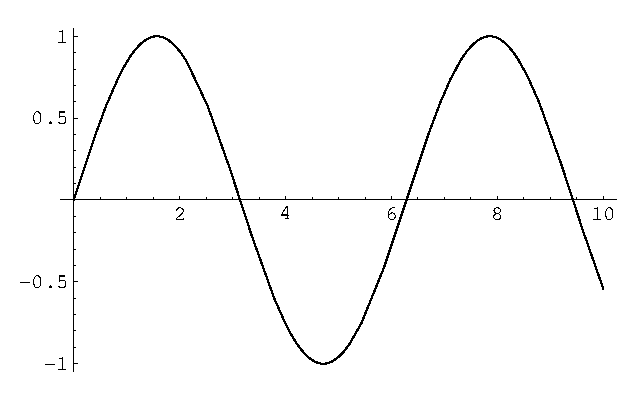
\includegraphics[width=5cm]{figures/mathematica}
\caption{Wykres.}\label{rys:plama}
\end{figure}

\begin{figure}[t]
\centering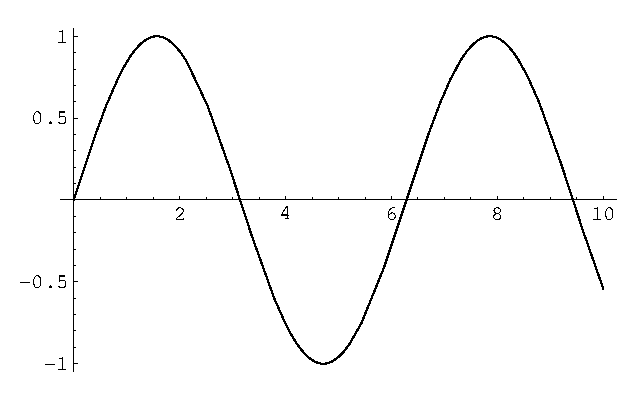
\includegraphics[width=\textwidth]{figures/mathematica}
\fcmfcaption{Ten sam wykres ale na szerokość tekstu. Formatowanie podpisu zgodne z wytycznymi FCMu.}\label{rys:plama2}
\end{figure}

Styl FCMu to nieco inne nagłówki rysunków. Dostepne są one poleceniem \texttt{fcmfcaption} (zob.~rysunek
\ref{rys:plama2}).

\subsection{Tablice}

Tablice to piękna rzecz, choć akurat ich umiejętne tworzenie w \LaTeX{}u nie jest łatwe. 
Jeśli tablica jest skomplikowana, to można ją na przykład wykonać w programie
OpenOffice, a następnie wyeksportować jako plik \akronim{PDF}. W każdym przypadku tablice wstawia się podobnie
jak rysunki, tylko że w środowisko \texttt{table}. Tradycja typograficzna sugeruje umieszczenie opisu tablicy, a więc
elementu \texttt{caption} ponad jej treścią (inaczej niż przy rysunkach).  

Tablica~\ref{tab:tabela} pokazuje pełen przykład.

\begin{table}[ht]
\caption{Przykładowa tabela. Styl opisu jest zgodny z rysunkami.}\label{tab:tabela}
\centering\footnotesize%
\begin{tabular}{l c}
\toprule
artykuł & cena [zł] \\
\midrule
bułka   & $0,4$ \\
masło   & $2,5$ \\
\bottomrule
\end{tabular}
\end{table}

Zasady FCMu sugerują nieco inne nagłówki tablic. Dostepne są one poleceniem \texttt{fcmtcaption} (zob.~tablicę
\ref{tab:tabela2}).

\begin{table}[ht]
\fcmtcaption{Przykładowa tabela. Styl opisu jest zgodny z wytycznymi FCMu.}\label{tab:tabela2}
\centering\footnotesize%
\begin{tabular}{l c}
\toprule
artykuł & cena [zł] \\
\midrule
bułka   & $0,4$ \\
masło   & $2,5$ \\
\bottomrule
\end{tabular}
\end{table}


\subsection{Checklista}

\begin{itemize}
\item Znakiem myślnika jest w LaTeXu dywiz pełen (---) albo półpauza (--), przykład:
  A niech to jasna cholera --- wrzasnąłem.

\item Połączenie między wyrazami to zwykły myślnik, przykład:   północno-zachodni

\item Sprawdź czy tutuł pracy ma maksymalnie dwa wiersze i czy stanowią one pełne frazy
  (czy nie ma przeniesienia bez sensu).

\item Sprawdź ostrzeżenia o 'overfull' i 'underful' boxes. Niektóre z nich można zignorować (spójrz
  na wynik formatowania), niektóre trzeba poprawić; czasem przeformułować zdanie.

item Przypisy stawia się wewnątrz zdań lub za kropką, przykład:
  Footnote is added after a comma.\footnote{Here is a footnote.}

\item Nie używaj przypisów zbyt często. Zobacz, czy nie lepiej będzie zintegrować przypis z tekstem.

\item Tytuły tabel, rysunków powinny kończyć się kropką.

\item Nie używaj modyfikatora [h] (here) do rysunków i tabel. Rysunki i tabele powinny być
  justowane do góry strony lub na stronie osobnej.

\item Wyróżnienie w tekście to polecenie \emph{wyraz}, nie należy używać czcionki pogrubionej (która
  wystaje wizualnie z tekstu i rozprasza).

\item Nazwy plików, katalogów, ścieżek, zmiennych środowiskowych, klas i metod formatujemy poleceniem
  \texttt{plik\_o\_pewnej\_nazwie}.

\item Po ostatniej zmianie do treści, sprawdź i przenieś wiszące spójniki wstawiając przed nie znak
  tyldy (twardej spacji), przykład:
  Ala i~kotek nie lubią mleczka, a~Stasiu lubi.
  
\item Za i.e. (id est) i e.g. (exempli gratia) stawia się zwyczajowo przecinek w typografii amerykańskiej.

\item Przed i za pełną pauza nie ma zwyczajowo spacji w typografii amerykańskiej, przykład:
  Darn, this looks good---said Mary.

\item Zamykający cudzysłów oraz footnote wychodzą za ostatni znak interpunkcji w typografii 
  amerykańskiej, przykłady:
  It can be called a ``curiosity,'' but it's actually normal.
  Footnote is added after a comma.\footnote{Here is a footnote.}

\item Odwołania do tabel i rysunków zawsze z wielkiej litery, przykład:
  In Figure~\ref{rys:plama} we illustrated XXX and in Table~\ref{tab:tabela} we show detailed data.
  
\end{itemize}


\section{Literatura i materiały dodatkowe}

Materiałów jest mnóstwo. Oto parę z nich:
\begin{itemize}
    \item \emph{The Not So Short Introduction\ldots}, która posiada również tłumaczenie 
    w języku polskim.\\
    \url{http://www.ctan.org/tex-archive/info/lshort/english/lshort.pdf}

    \item Klasy stylu \texttt{memoir} posiadają bardzo wiele informacji o składzie tekstów
    anglosaskich oraz sposoby dostosowania \LaTeX{}a do własnych potrzeb.\\
    \url{http://www.ctan.org/tex-archive/macros/latex/contrib/memoir/memman.pdf}
    
    \item Nasza grupa dyskusyjna i repozytorium Git są również dobrym miejscem aby zapytać
    (lub sprawdzić czy pytanie nie zostało już zadane).\\
    \url{https://github.com/politechnika/put-latex}

    \item Dla łaknących więcej wiedzy o systemie LaTeX podstawowym źródłem informacji
    jest książka Lamporta~\cite{Lamport1985}. Prawdziwy \emph{hardcore} to oczywiście
    \emph{The \TeX{}book} profesora Knutha~\cite{Knuth1986}.
\end{itemize}



%--------------------------------------
% Informacja o prawach autorskich
%--------------------------------------

\ppcolophon

\end{document}